\chapter{Results and Discussion}
In this chapter, we describe and discuss the results of this project.
In first section, we present implementation of the pipeline allowing us to transform the raw protein sequences from FASTA format into the input format of the neural network.
Then, in the second section, we reveal the networks used to predict the distograms of the proteins.
We also discuss the experiments done to confirm the correctness of our implementations and compare different architectures.
The last section is dedicated to constructing the 3D structure from these predicted distograms.

\section{Pipeline}

\begin{figure}
    \centering
    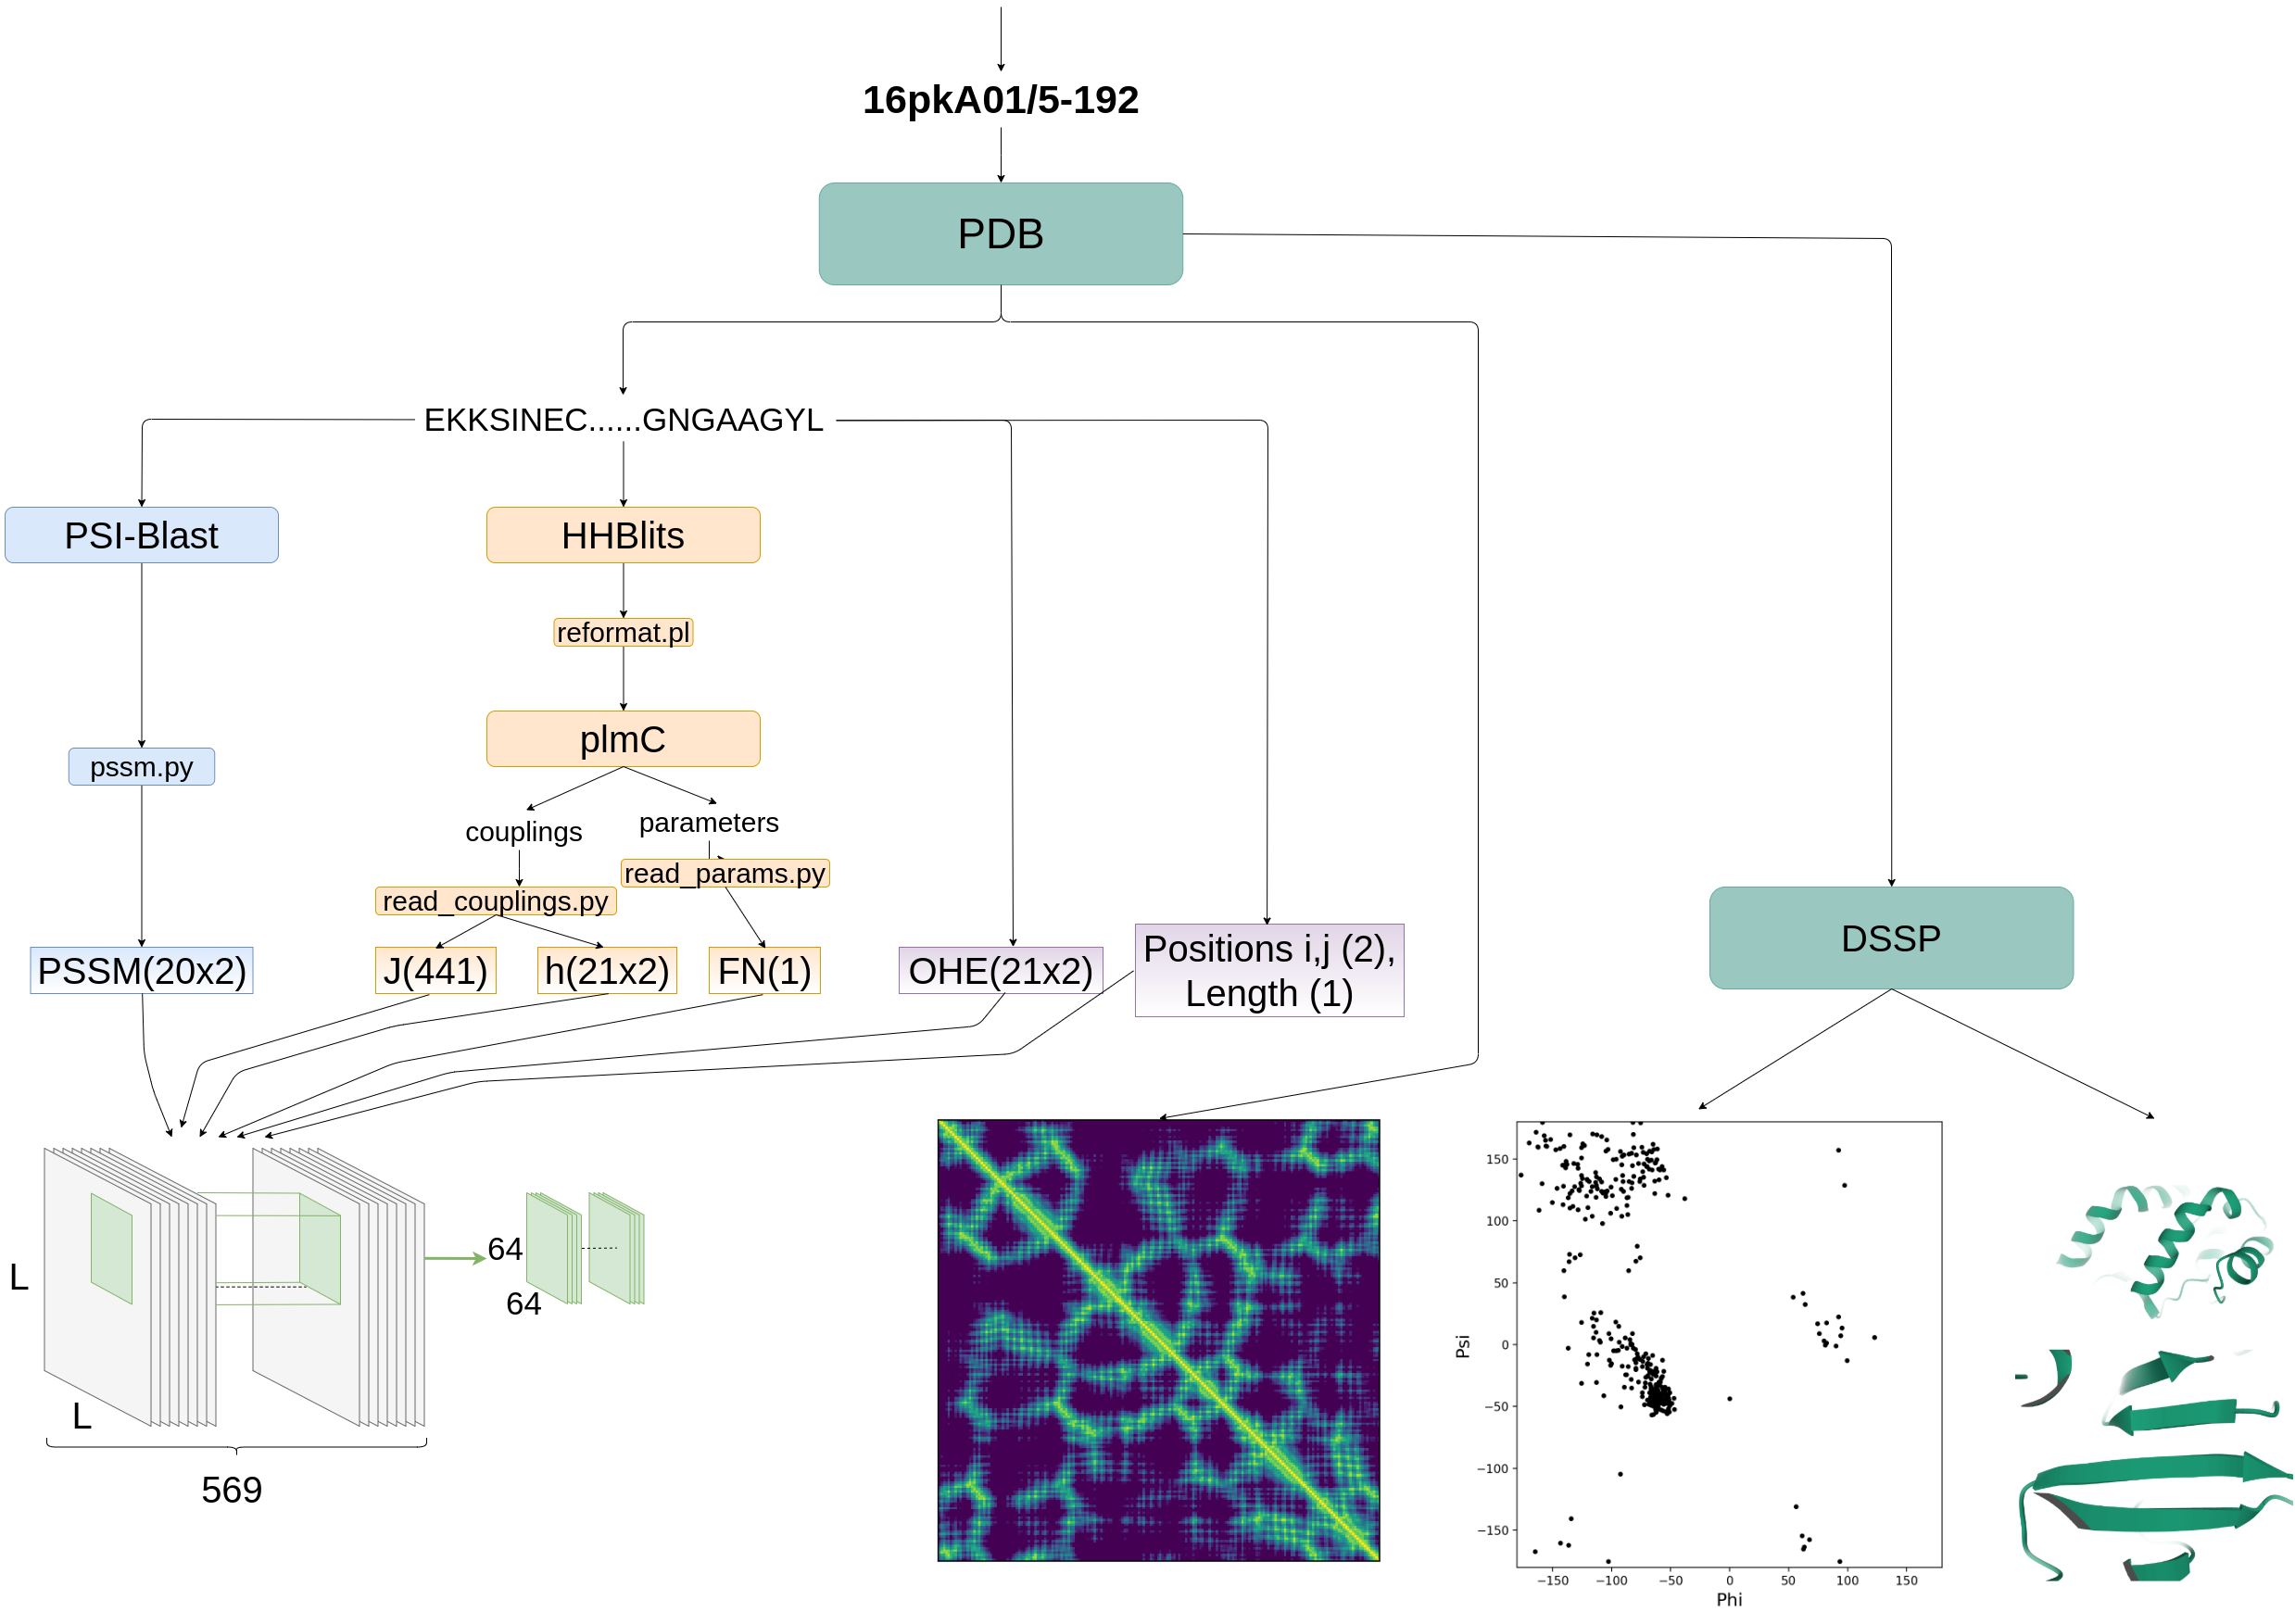
\includegraphics[width=\linewidth]{imgs_tomas/pipeline_input.png}
    \caption{Input / Output data generation}
    \label{fig:pipeline_input}
\end{figure}

The pipeline was constructed to formalize and automate the process of data preparation for the neural networks.
It was written in \texttt{Snakemake} workflow management system \cite{koster2012snakemake}, which is highly popular in the bioinformatics field with approximately 3 new citations every week.
The workflows consist of rules, which define the data dependency in the form of rule input files, rule output files and the script, which needs to be executed to get from input to output. 
This definitions make using of \texttt{Snakemake} very convenient.
The rules are defined as a subset of YAML, extended by the option to run python code directly, which makes them easily readable by humans.
The structuring of the workflow allows seamless scalability to server environments and parallelization to multiple cluster nodes and multiple cores.
This capability was very crucial for this project due to the amount of data available.
Furthermore, \texttt{Snakemake} automatically checks for completed rules, which is in turn used to run only the rules needed for the defined target.
It also checks the exit code of the scripts and informs the user if there is an error during the execution and therefore decreases a chance of working with faulty data to the minimum.
Finally, \texttt{conda} \cite{conda}, the package management system, is nicely integrated into \texttt{Snakemake}, which simplifies the installation of most packages and bioinformatics tools needed during the analysis.
It is also possible to fix package versions used during the analysis, which hugely improves reproducibility.
Next, we present the main steps in the pipeline.
The complete pipeline can be found on our GitHub repository \cite{github}.

\subsection{PSI-BLAST}
The first step in the pipeline was the construction of the PSSMs of the protein sequences.
For this purpose, we used the PSI-BLAST \cite{altschul1997gapped}, an improved variation of the BLAST algorithm focused on PSSM construction.
The PSI-BLAST first identifies proteins similar to our query protein from the database above a certain threshold.
The threshold is inversely proportional to an E-value, which represents the number of expected hits in a database of a particular size just by random chance.
In our project, we used a default \texttt{E-value} of 10.
The proteins identified as similar are then aligned to the query protein.
Proteins with an insufficient alignment score are discarded from the set of similar proteins.
Here, the parameter \texttt{-inclusion\_ethresh} is used to determine which alignments should be included in the set. 
Afterwards, the MSA is constructed from the set of similar proteins and the PSSM profile is calculated from this MSA.
The PSSM profile is then used to identify proteins corresponding to this profile, similarly as the original sequence was used.
A new PSSM profile is then calculated using these newly identified proteins.
This process is iterated multiple times, improving the PSSM each iteration as was shown in Altschul et al. \cite{altschul1997gapped}.
In our implementation, we used 3 iterations to construct the final PSSM. 
The PSI-BLAST algorithm is sketched out in Figure \ref{fig:psi_blast}
\begin{figure}
    \centering
    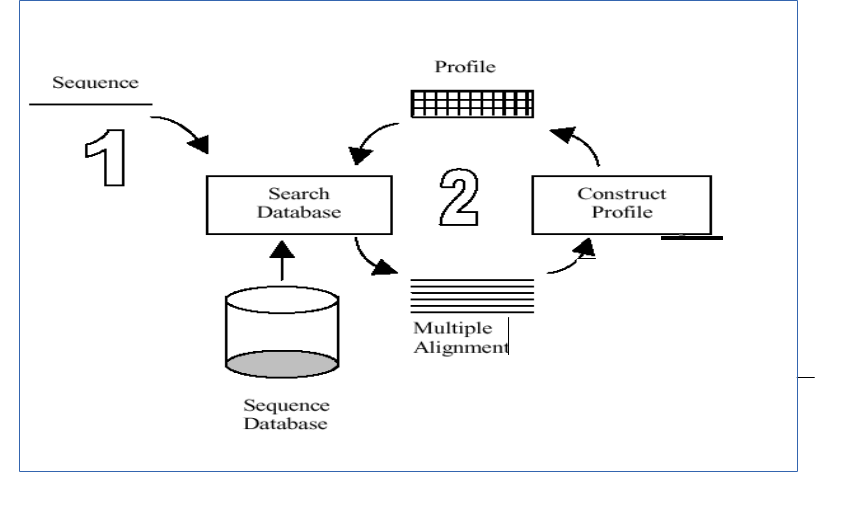
\includegraphics[width=\linewidth]{imgs_andy/psi_blast.png}
    \caption{PSI-BLAST process}
    \label{fig:psi_blast}
\end{figure}

\subsection{HHblits}
Another step, parallel with the PSI-BLAST step was the construction of MSA using HHblits \cite{remmert2012hhblits}.
This MSA was later used as an input to the Potts models.
The HHblits takes a slightly different approach to MSA construction than the PSI-BLAST, which we considered an advantage because the correlation of the input features to the neural networks was decreased.
The HHblits first converts the query sequence to a Hidden Markov Model (HMM), which is then compared to HMMs from the database.
The database HMMs below a certain E-value threshold are then added to the query MSA, from which a query HMM for the next iteration is constructed.
This process is then repeated defined number of times.
In this project, we used E-value of 0.001 and 3 iterations to arrive at the final MSA.

\subsection{plmc}
To create Potts models from the MSA, we used a plmc software from Debora Marks Lab \cite{plmc}.
Given the MSA in FASTA format, the software produced two files: "couplings file" containing Frobenius norm of the $\bm{J}$ matrix and an optional binary "param file" containing the full $\bm{h}$ and $\bm{J}$ tensors. 
The plmc software used the second-order optimization algorithm LBFG-S to iteratively fit these parameters.
The number of maximum iterations used in our pipeline was set to 500 \cite{plmc}.

\subsection{Input encoding}
The last step of the input preparation pipeline was to create an input tensor for the neural networks.
We used the input tensor of size $L \times L \times C$, where $L$ is the length of the protein sequence and $C$ is the number of channels.
To create such tensor, we used the Potts model parameters, one-hot encoded protein sequence and the PSSM profile.
We also added channels representing positions and the length of the protein.
The complete description of the input tensor was as follows.

\begin{itemize}
    \item Potts model's pairwise interactions $J$ transformed from size $L \times L \times 21 \times 21$ to $L \times L \times 441$
    \item Frobenius norm of pairwise interactions $J$ of size $L \times L \times 1$
    \item positions from $0$ to $L-1$ transformed from size $L \times 1$ to $L \times L \times 1$
    \item Potts model's propensities $h$ transformed from size $L \times 21$ to $L \times L \times 21$
    \item one-hot encoded protein sequence transformed from size $L \times 21$ to $L \times L \times 21$
    \item PSSM profile transformed from size $L \times 20$ to $L \times L \times 20$
    \item tensor of size $L \times L \times 1$ containing a constant value of protein length
\end{itemize}

The positions, Potts model's propensities $h$, one-hot encoded protein sequence and PSSM profile were simply repeated $L$ times along the axis to match the required size.
Both, repetition along the first and second axis, were used, therefore the resulting number of channels $C$ was $441 + 1 + 2 \cdot 1 + 2 \cdot 21 + 2 \cdot 21 + 2 \cdot 20 + 1 = 569$. 

\subsection{Data}

\begin{figure}
    \centering
    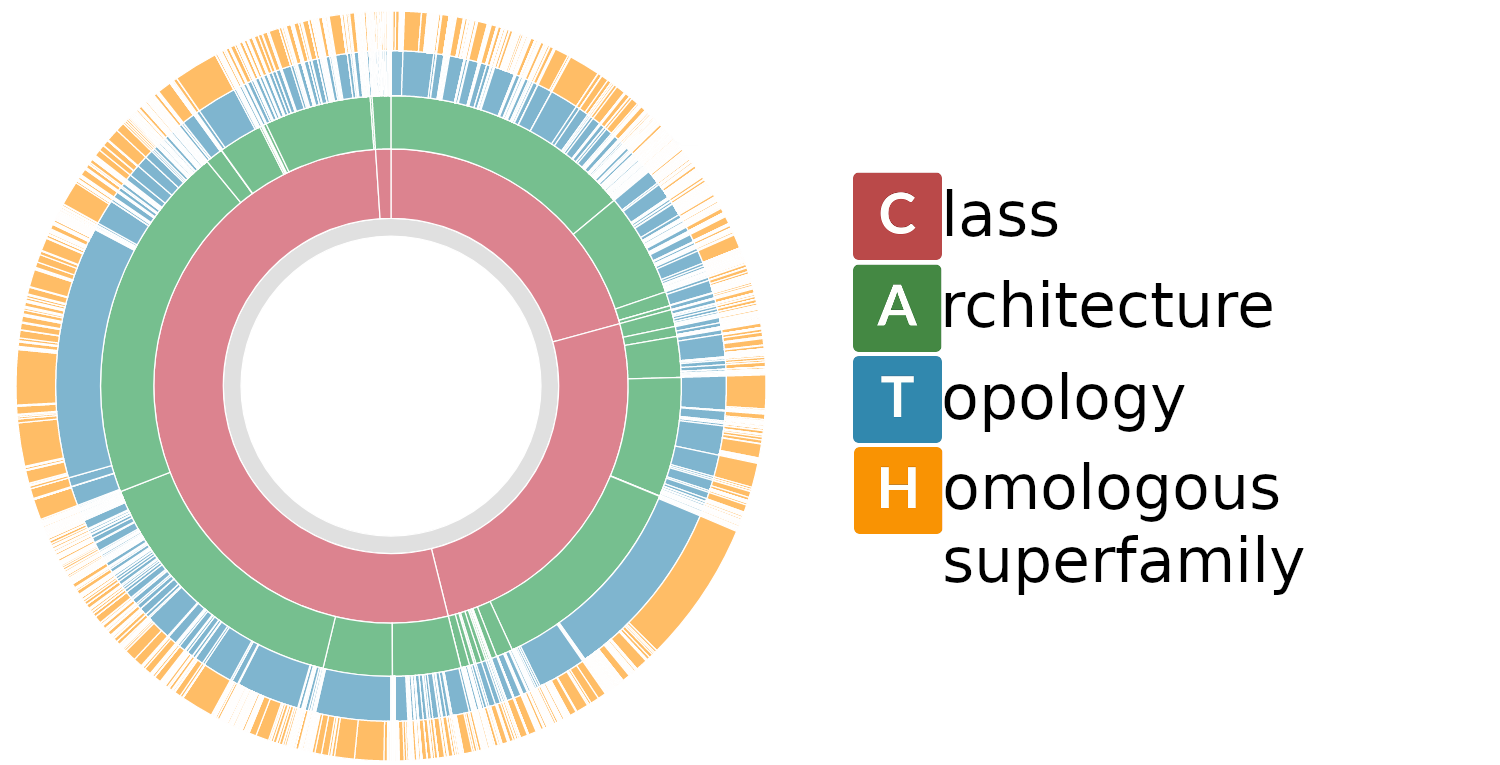
\includegraphics[width=\linewidth]{imgs_tomas/cath.png}
    \caption{CATH hierarchy \cite{cath}}
    \label{fig:cath}
\end{figure}

For training and evaluation of models, it is important to use diverse data sets, that capture a wide range of different scenarios and thus force the model to generalize well. For this reason, a CATH dataset was created.
CATH is a database that clusters proteins with known structures based on 4 criteria: Class (secondary structure classes), Architecture (secondary structure arrangement in 3D space), Topology (how secondary structure elements are connected) and Homologous Superfamily (the evolutionary relationship between domains). 
Figure \ref{fig:cath} shows the hierarchical relationship between the classes.
    
To ensure dataset diversity, we used a dataset of sequences with pairwise sequence similarity of at most 35\%. 
The list of domains together with their sequences in \texttt{fasta} format can be accessed at: \href{ftp://orengoftp.biochem.ucl.ac.uk/cath/releases/latest-release/sequence-data/cath-domain-seqs-S35.fa}{oregonftp.biochem.ucl.ac.uk}.

Domains are short regions of proteins that fold more or less independently of each other. 
The \texttt{fasta} file contains for each domain its protein name, chain identifier and the domain ranges. 
This information is crucial for downloading and preparing the structures from the Protein Data Bank database. 
Two example headers are shown below. 
    
\begin{center}
    \texttt{>cath|4\_2\_0|1a41A02/217-310}\\
    \texttt{>cath|4\_2\_0|3lnnA01/12-42\_283-342}
\end{center}
    
These two examples show domains - \texttt{1A41} and \texttt{3LNN}, downloaded from the CATH database version 4.2.0. 
The next letter (\texttt{A} in both cases) represents the chain and the last two characters are the domain id since a chain can consist of several domains. 
The full dataset (version from Sept. 4 2017) consists of 31289 domains. 
    
We decided to exclude segmented domains from the dataset and also the ones with missing PDB coordinates. 
This resulted in a set of 19953 domains. 
Looking at the sizes of homologous superfamilies in Figure \ref{fig:cath}, there are few large ones (like the immunoglobulin family in the bottom right corner with more than 8000 domains) and the rest are relatively small (less than 50). 
Our model works with evolutionary data (MSA - PSSMs/Potts), which means that having an over-represented family in the data set might introduce some biases that might make the model generalization more difficult. 
For this reason, we decided to impose an exclusion threshold (= 500), wherein families with more members we randomly picked "exclusion threshold" of domains out of them. 
After this filtering, the dataset size reduced to 11014 domains.
The distributions of CATH classes after filtering can be seen in Figure \ref{fig:cath_filtered}.
    
\begin{figure}
    \centering
    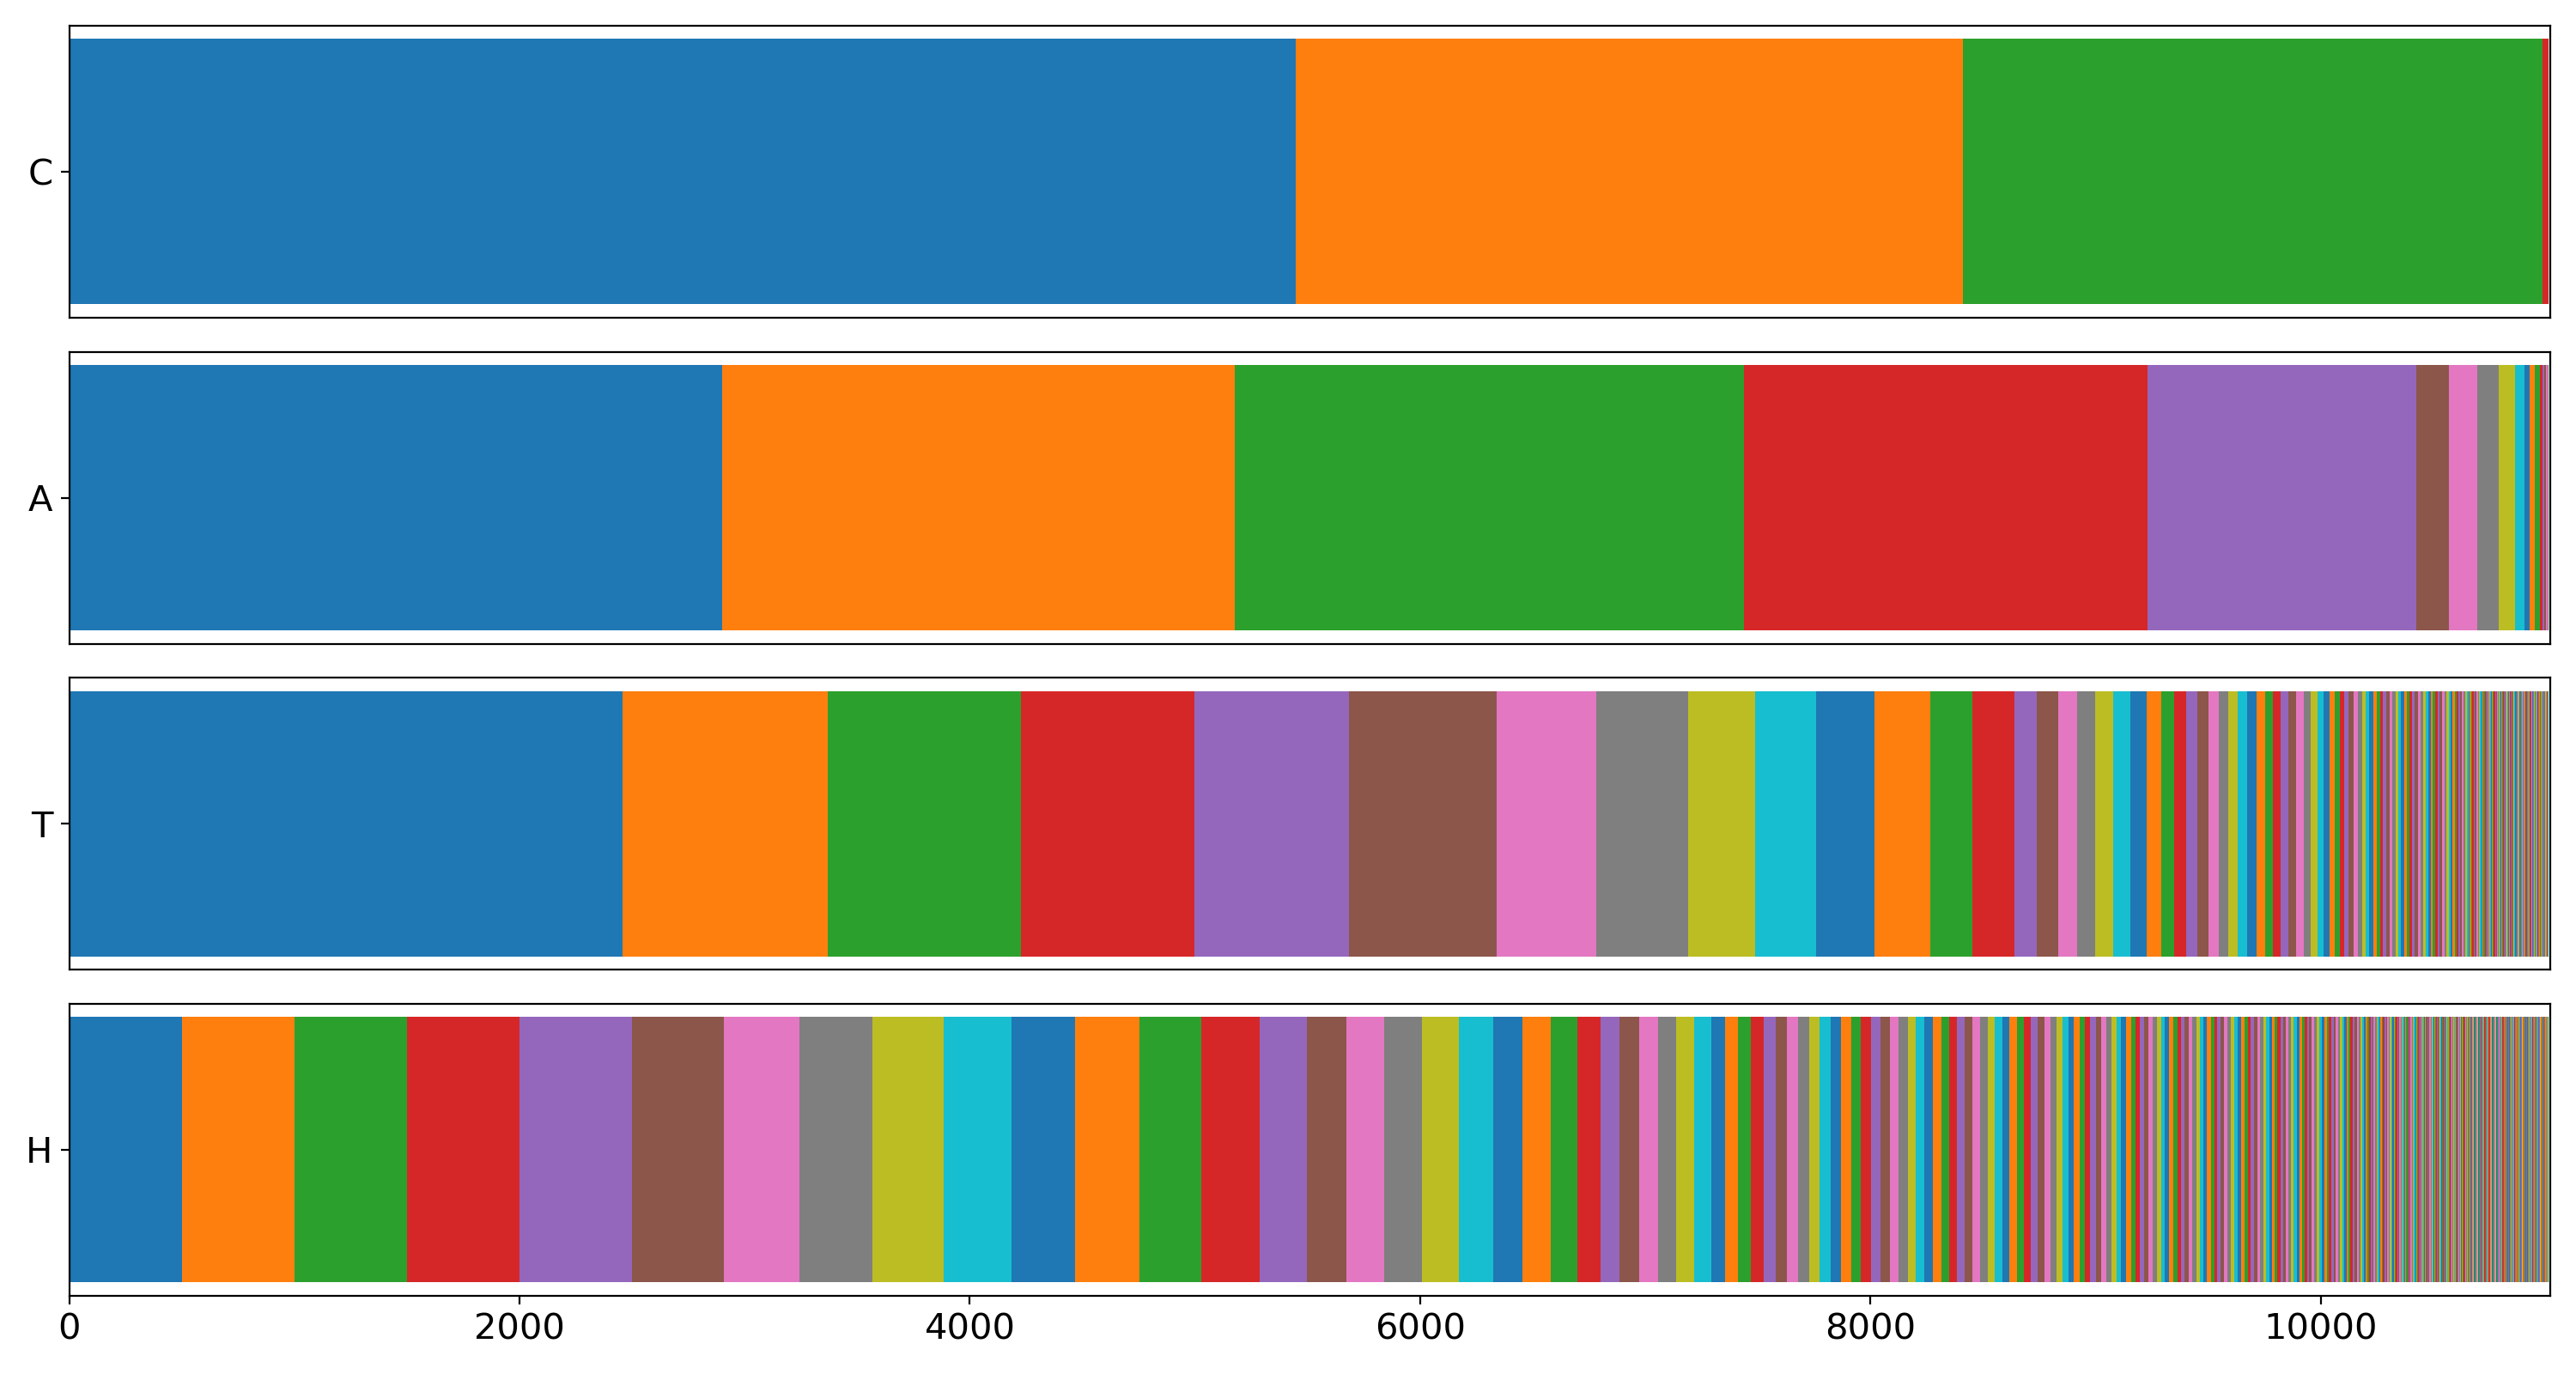
\includegraphics[width=\linewidth]{imgs_tomas/cath_distributions_filtered.png}
    \caption{CATH families distributions after filtering out over-represented homologous superfamilies, removing segmented domains and removing domains with missing PDB coordinates}
    \label{fig:cath_filtered}
\end{figure}

\subsection{Output encoding}

The labels used for training were downloaded from the Protein Data Bank (PDB) which offers a rich description of proteins, including their tertiary structure. 
Domains with missing coordinates were filtered out of the dataset.
        
Although the distance is a continuous measure, and it would make perfect sense to treat the problem as a regression one, AlphaFold discretized the distances into 64 bins ranging from 2 to 22\AA, with one bin used for distances larger than 22\AA and one bin for missing data (in our case a zero-padding label). 
The reason for doing so becomes clearer after understanding how the structure realization (the last step of the entire pipeline) was performed.

To make the task slightly simpler for the neural network, we binned the distances into 32 bins (with the first bin - bin 0 used for missing values/padding and last bin for distances larger than 22 \AA).
        
The secondary structure was classified into 9 categories (padding label + 8 DSSP classes) suggested by DSSP (Dictionary of Protein Secondary Structure) \cite{dssp1, dssp2, dssp3}.
The categories are shown in table \ref{tab:dssp0}.

On top of the secondary structure classification, the output of the DSSP program also conveniently includes the torsion angles $\phi$ and $\psi$. These were categorized to 37 bins (padding label + bin for every 10\degree).

\subsubsection{Train/Validation/Test split}

\begin{figure}
    \centering
    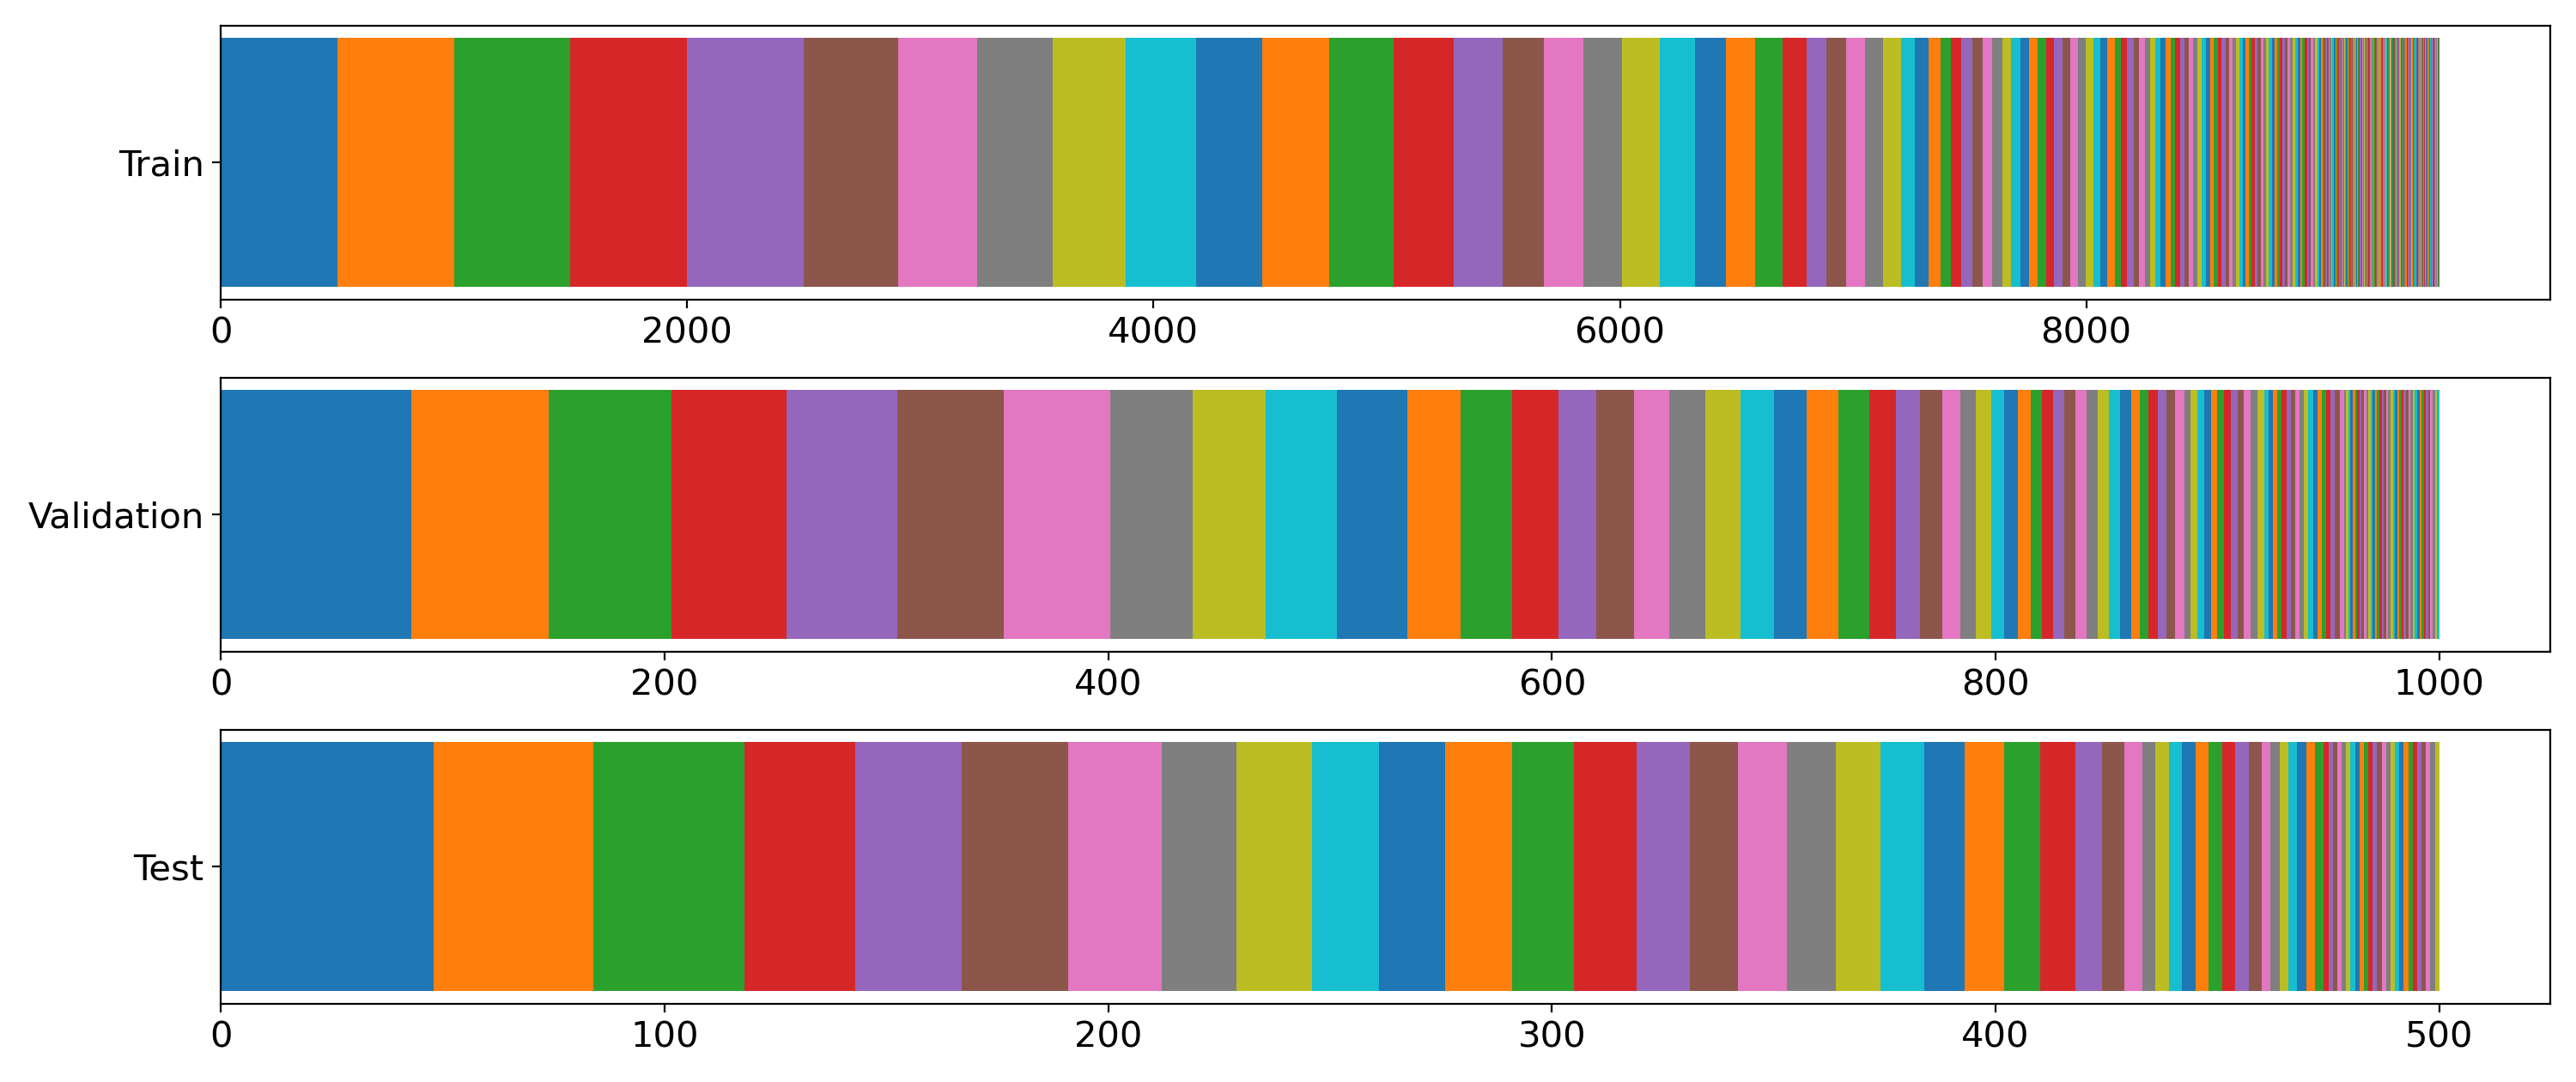
\includegraphics[width=\linewidth]{imgs_tomas/cath_distributions_trainvaltest.png}
    \caption{Representation of homologous superfamilies in Train, Validation and Test set. (The colours do not correspond to the same superfamilies, they simply divide the superfamilies in each row)}
    \label{fig:cath_trainvaltest}
\end{figure}

Following the example of AlphaFold \cite{alphafold}, we decided to create a train/validation/test set of homologous superfamilies instead of randomly sampling domains. 
The rationale behind this is to include all members of each homologous superfamily in either training, validation or test set. 
This ensures that when evaluating the model performance on a set of proteins, those very similar proteins were not used for training. 
    
We decided to train our models on a set of 9394 domains (several had to be excluded due to factors such as low sequence similarity to known structures or inability to converge/slow convergence of the Direct Coupling Analysis). This set of domains was used to train the neural networks and for the estimation of the loss during the training process.

The performance of the different models was evaluated on an independent validation set of 1000 domains. For each model, we evaluated its inter-residue distance predictions as well as the auxiliary outputs (secondary structure and phi and psi torsion angles).

The final structures and performance metrics were evaluated on a set of 500 test domains.
    
Furthermore, to simulate the famous CASP competition we downloaded 13 domains from CASP13 (2018) - regular targets category (T). This allowed us to compare our results with the best teams in the world.

\newpage
\section{Inter-residue distance modelling}

For the past couple years, one way of evaluating similarity between real and predicted structures, was to look at their contact maps. Residue-residue contact is a binary feature that describes whether the C$_\alpha$ (or C$_\beta$) atoms of two residues are closer to each other than 8\AA. Several softwares, such as CONFOLD2 \cite{confold, confold2} were developed to use the contact maps as constraints for structure modelling. The potential of using contact maps for modelling was shown on CASP12 and CASP13, where the contact precision reached ~47\% and ~70\% respectively (before, the average contact precision was between 20-30 \%). Although this progress, there is a limit on how good the predictions can be (the authors of CONFOLD2 report average TM-score of 0.57 \cite{confold2}). For this reason several teams on CASP13, AlphaFold included, decided to predicted inter-residue distance distributions and use them as constraints for structure optimization. This has shown a great potential, especially after noticing that AlphaFold was ranked first for many of the targets (including hard ones).

The reason behind the substantial increase in contact predictions is mainly due to the use of deep neural networks. Neural networks (thoroughly described in the methods section) are incredibly versatile family of models. Since our input and output were essentially 3 dimensional tensors, the convolutional networks are a reasonable architecture choice. 

In the next subsection we describe the main architecture of the network used for predicted distance histograms + auxiliary outputs together with description of 3 different modules that were tested. The second subsection describes the training strategy and third one evaluates the performance of the models.

\subsection{Neural Networks}
% architectures (convnet, Alphafold, Inception), training, auxiliary losses, ...

\begin{figure}
    \centering
    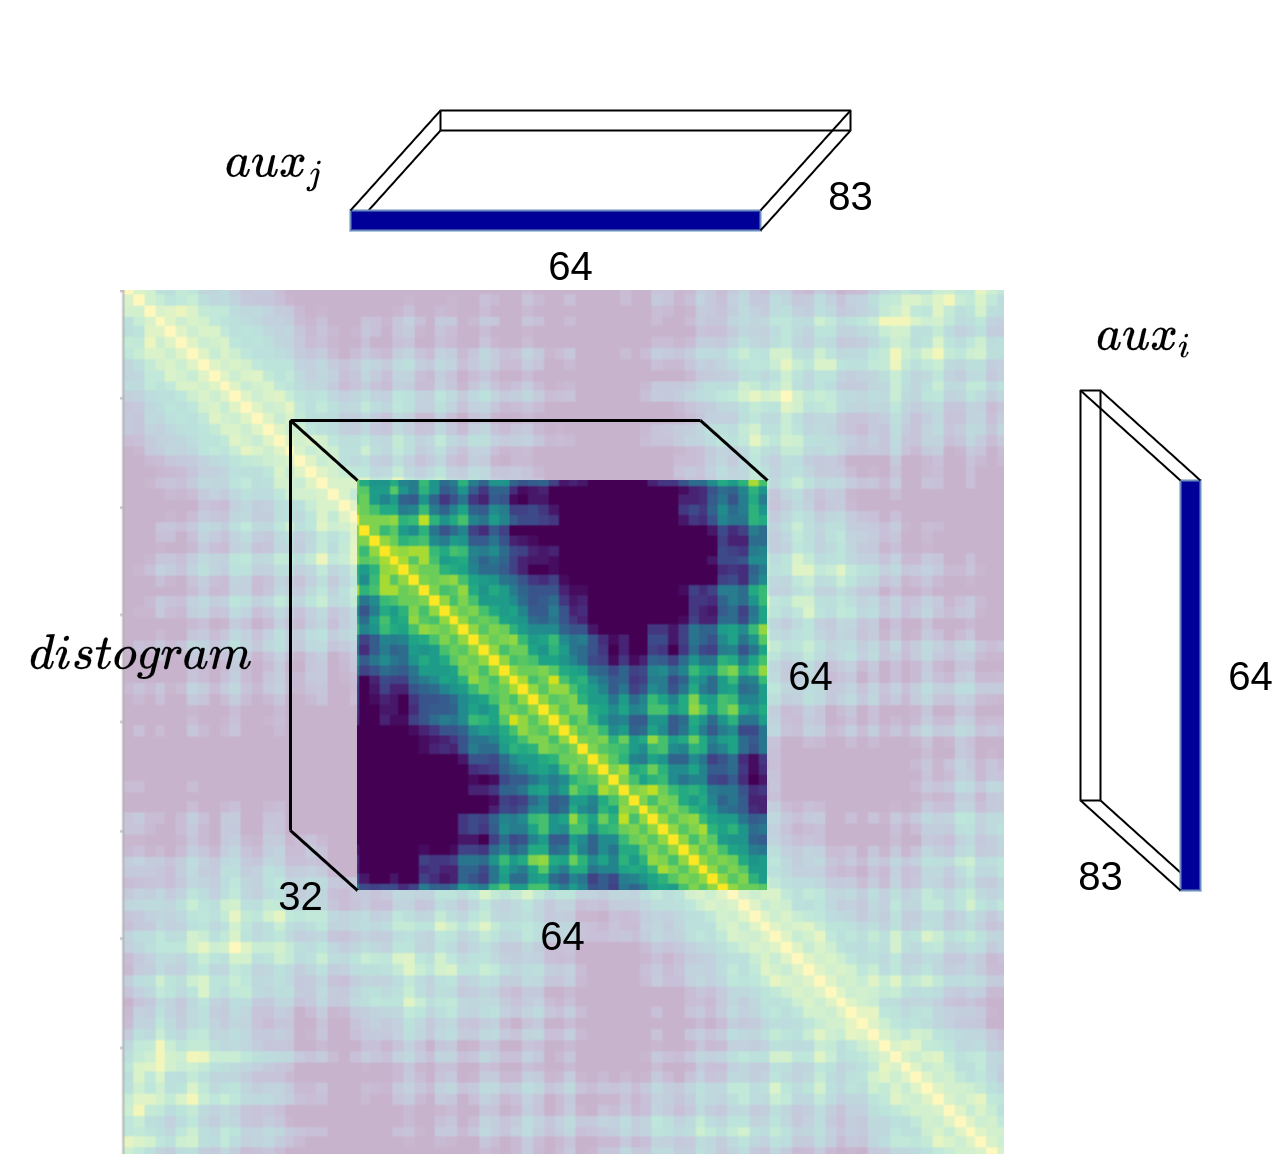
\includegraphics[width=0.7\linewidth]{imgs_tomas/outputs.png}
    \caption{Neural network distogram and auxiliary outputs with corresponding dimensions}
    \label{fig:outputs}
\end{figure}

Before diving to the specifics of each module, we have to explain the overall/general architecture shared between the models (see Figure \ref{fig:architectures}a)). The first crucial thing to keep in mind, is to ensure that the dimensionality of the input does not change throughout the network, since our labels were 2D (binned) distance maps. This means that no pooling operations are allowed, only convolutions without changing the dimensionality. The layers inside the networks are thus essentially only of three types: convolutional (1x1, 3x3, 5x5, 64x1, dilated, ...), Batch norm and Elu/Relu layers. The only difference between the individual modules is in the number of these layers and their arrangement.

In order for the input features to be roughly on the same scale, the first layer of the network is a Batch normalization one. As the number of channels in the input was 569, the second layer decreases this number by applying the 1x1 convolution. Its output is then fed through a series of modules (described more thoroughly in later paragraphs).

The end of the network branches into two output heads: distogram head, which decreases the number of channels to 32 and auxiliary head that applies two convolution operations, to arrive at 2D input with 84 channels (9 channels for secondary structure, 37 channels for phi angle and 37 channels for psi angle) - see Figure \ref{fig:outputs}. The "$aux_j$" output was taken directly after applying the 64x1 convolution and $aux_i$ output was taken as a transpose of the same layer. In a way this created two auxiliary heads with shared weights. The entire architecture together with the modules described below is shown on Figure \ref{fig:architectures}.

\begin{figure}
    \centering
    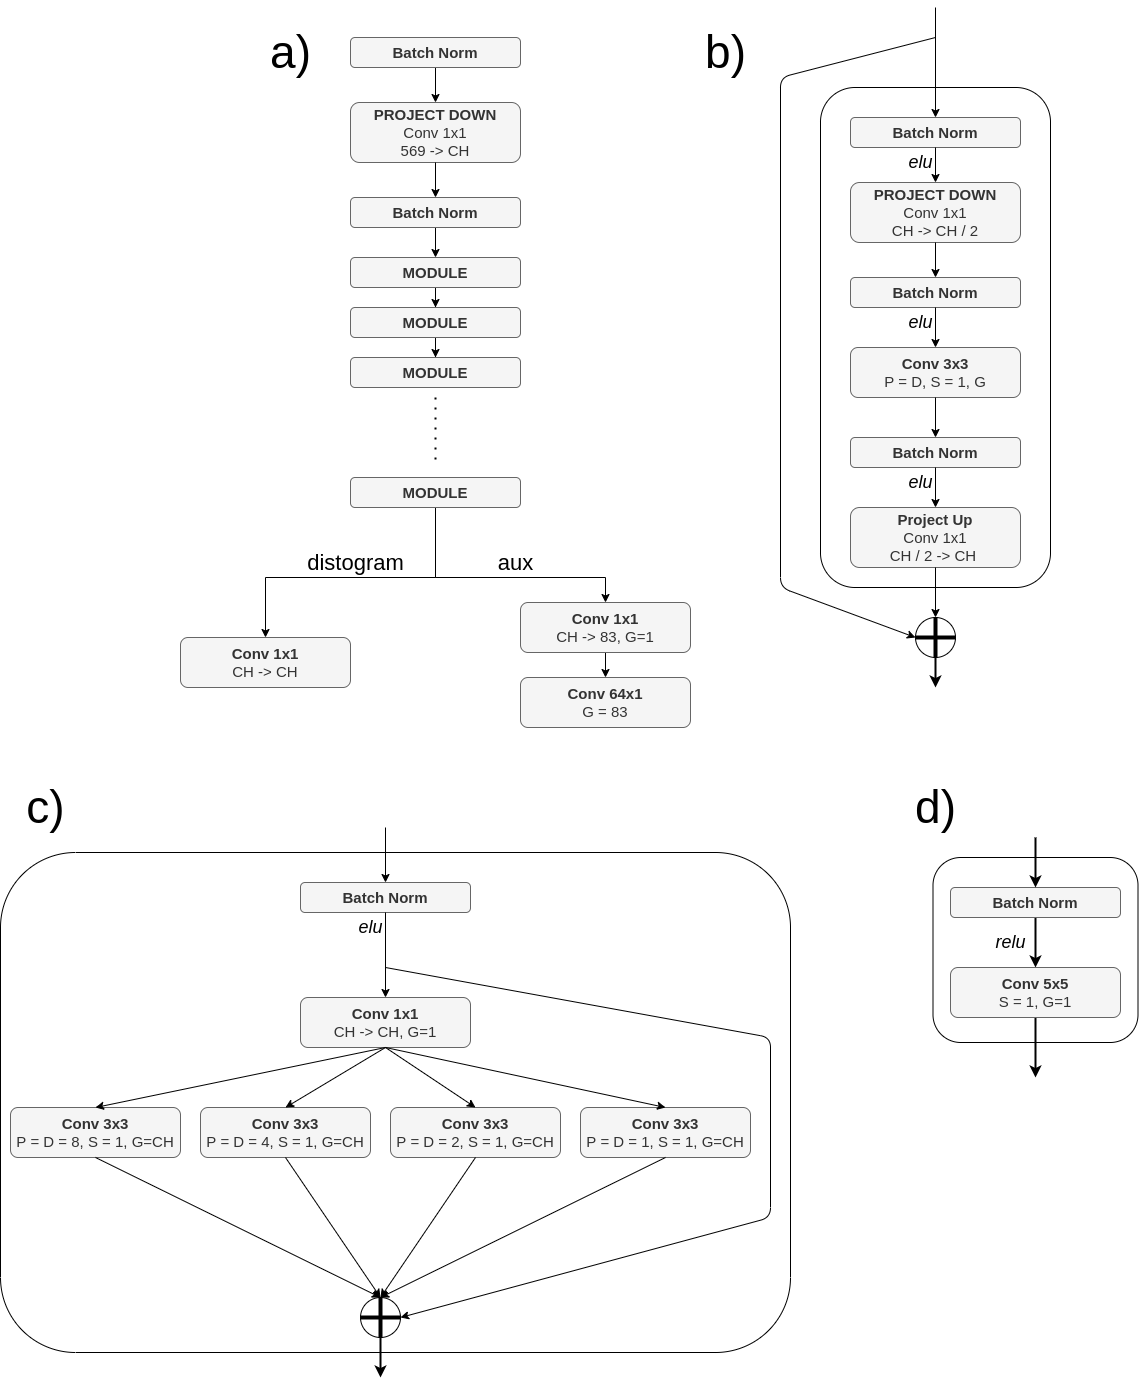
\includegraphics[width=\linewidth]{imgs_tomas/Architectures.png}
    \caption{Neural Network architectures used in training. a) visualizes the diagram of the entire network; b) shows the AlphaFold block, c) is an Inception Resnet module (inspired by Inception module used in GoogleNet \cite{googlenet}) and d) is a simple Convolutional Network}
    \label{fig:architectures}
\end{figure}

\subsubsection{ConvNet}

We begin with a simple convolutional network. The network consisted of 16 modules, each one applying a Batch Norm operation and a 5x5 convolution (with stride=1, padding=2, groups=1) - see Figure \ref{fig:architectures} d). This might not seem like a simple network, but the reasoning behind the number 16 follows from the definition of the local receptive field (LRF). LRF describes area of the input that is captured by a neuron in a convolutional layer. When successively applying the 5x5 convolutions, this area increases by 4 in each dimension (5x5, 9x9, 13x13, ...). Thus, since the size of the input was fixed at 64x64 (see cropping schemes in training section below), the minimal number of layers needed so that each neuron captures the entire input is 16.

The number of channels inside the network was fixed at 128 and the activation function applied between modules was relu. All in all, the number of parameters of the network was 6,654,328.

\subsubsection{AlphaFold}

For notational purposes, we are going to distinguish three features of the network: the AlphaFold block, the Alphafold Module and AlphaFold network.

The main feature of the alphafold resnet block (depicted on Figure \ref{fig:architectures}b)), are the dilated 3x3 convolutions. It begins with a Batch norm layer, followed by a 1x1 convolution layer decreasing the number of channels to one half. After applying another batch norm layer comes the dilated 3x3 convolution. The size of the dilation was picked from a list: \{1, 2, 4, 8\}. The block is concluded with a Batch norm layer followed project up layer, that restores the number of channels so that they can be added to the input. The activation function used between the layer was elu.

The Alphafold module consisted of 4 Alphafold blocks cycling through 4 different dilations. We built two versions of AlphaFold network: one with 40 modules with number of channels = 128 and applying 3x3 convolutions with groups = 128, and another one with first 4 modules having 216 channels and then 32 modules with 128 channels applying convolutions with groups=1. In further text we will refer to the first network as Alphafold and second as Alphafold\_ZP (due to the cropping scheme strategy involving Zero Padding). 

All in all, the number of parameters in Alphafold was 3,639,928 and in Alphafold\_ZP 10,745,464. This difference is mainly the result of applying 3x3 convolutions in the blocks channel wise ($\Longleftrightarrow$ groups = channels).

\subsubsection{Inception}

The name of the Inception Network %suggests, that there is a network inside a network.
comes from an architecture presented by team Google at ImageNet 2014, where it consisted of a "network of networks".
This becomes more obvious after inspecting the Inception Resnet Module in Figure \ref{fig:architectures}c). GoogleNet (name of the entire model) won the competition while showing great potential of 1x1 convolutions.

The module starts off with a batch norm layer, than applies 1x1 convolutions and finally branches into four 3x3 dilated convolutions (dilations = \{1, 2, 4, 8\}) which are added in the end with the input. This step also makes it a Residual Network.

The activation function used in intermediate layers was elu and the number of channels was kept at 128.

The idea behind this module is to let the network to pick a "path" depending on the required level of detail. This way one can capture general variation while taking the path through more dilated convolutions while focusing on more details with smaller dilations \cite{nn_dl}.

\subsection{Training Strategy}

\subsubsection{Cropping}

The cropping refers to a process in which % we sliced a region of the size
a sliced region of shape $\text{crop\_size} \times \text{crop\_size}$ is extracted from the input of size $L \times L$. In our pipeline (as was done in AlphaFold) we used crops of size 64x64.
These crops were then used for neural network training, as well as for predicting novel data. This step was necessary and beneficial for following reasons: 

%The sliced region was then used to train the neural network.
%This process served multiple purposes.
\begin{enumerate}
    \item Independence from input size ($\Leftrightarrow$ domain length)
    % It allowed us to use the network %across all proteins with differing lengths. 
    % without caring about the size of the input ($\Leftrightarrow$ domain length).

Although the convolution operation can be used on input of different sizes, one of the last steps in our networks was to predict auxiliary losses of secondary structure and torsion angles.
For this, we needed to reduce the multiple 2D maps into 1D maps, which was achieved by applying convolution with kernel size $1 \times \text{crop\_size}$.
%This meant to reduce the multiple 2D maps into multiple 1D maps.
%For this purpose, we used the convolution with a kernel of size $1 \times \text{crop\_size}$.
If it were not for the unified size of the input, we would need to use kernel size of $1 \times L$, which is different for all proteins and therefore we would not be able to reuse the same parameters for auxiliary loss prediction.

    \item Data augmentation
    
During every epoch, the crops were randomly offsetted and then fed to the network. This means that for every iteration the network needs to predict certain region with slightly different input data at hand, which forces it to generalize better.
% add some description why?

    \item Memory load and the time consumption decrease during training
    
    

% add some description why?
% add more advantages?
\end{enumerate}

%During the training, 
We experimented with two cropping schemes.

In the first cropping scheme, we only considered the inner crops.
First we selected offsets $O_x, O_y$ for the x-axis and for the y-axis respectively. 
This offsets were random integers from the interval $[0, 63]$.
Then, we constructed crops across all domains loaded in RAM and across all channels of these domains.
Position of these crops was from $O_x$ to $O_x + 64$ along the x-axis and from $O_y$ to $O_y + 64$ along the y-axis.
If the crops were out of bounds of the domain ($O_x + 64 > L$ or $O_y + 64 > L$), then we discarded them as we did not consider them to be a valid crops.
Next, we trained our model in batches of 8 valid crops at a time.
Afterwards, we created another crops out of region from $O_x + 1 \cdot 64$ to $O_x + 1 \cdot 64 + 64$ along the x-axis and from $O_y + 0 \cdot 64$ to $O_y + 0 \cdot 64 + 64$.
We continued the training and cropping along the x-axis until starting coordinate of x offset were smaller the the biggest length of the loaded domains.
Then, we shifted the crops along the y-axis, so the y offset was $O_y + 1 \cdot 64$.
We continued this cropping process until we covered all inner crops of the longest domain.
This cropping scheme is visualized in Figure \ref{fig:cropping} a).

The second cropping scheme (visualized on Figure \ref{fig:cropping} b)) - also used by Alphafold, allows the crops to go "outside" of the input. The excess regions are represented with number 0 together with a label of the same number. The zero padding never exceeded length of 32, meaning that at least 32x32 region of the input was always included inside of the crop (the shape of crops was 64x64). The crops were non-overlapping and some degree of freedom (dependent on the size of the input) regarding the offset of the entire crop map (orange squares on Figure \ref{fig:cropping} b)) allowed us to feed the network with diverse data while training. The zero padding also allowed us to train on domain shorter than 64 residues, which is not possible with the first cropping scheme.

\begin{figure}
    \centering
    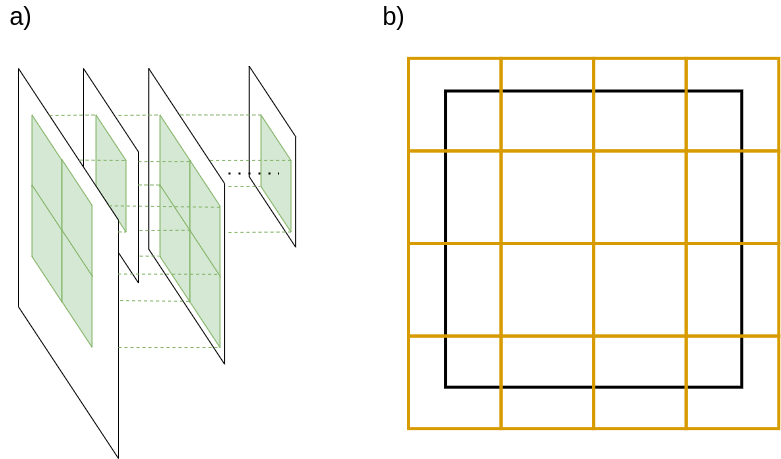
\includegraphics[width=\linewidth]{imgs_tomas/cropping_schemes.png}
    \caption{Two Cropping strategies used for training the networks. a) shows the cropping strategy used to train model named Alphafold, while the rest models (and also the original Alphafold \cite{alphafold}) used the second strategy b)}
    \label{fig:cropping}
\end{figure}

\subsubsection{Training}

The training involved 3 stages: loading input data, cropping and applying gradient descent steps.

It was not possible load all data in memory (the occupied space $\approx$ 1TB), so the data loading and training was performed on smaller chunks of the data. We loaded the input tensors in parallel, which increased the training speed substantially.

Then a bank of crops of sizes 64x64x569 was created which was fed to the network in batches of size 8. We used weighted negative log likelihood as the loss function to give more importance to the distance predictions than auxiliary losses. Formally:

\begin{equation}
    NLL = 10 \cdot NLL_{dist} + NLL_{sec_i} + NLL_{sec_j} + NLL_{\phi_i} + NLL_{\phi_j} + NLL_{\psi_i} + NLL_{\psi_j}
    \label{eq:NLLloss}
\end{equation}

The train loss was calculated on a set of domains used in training and validation loss on a held out set. 

We saved intermediate models (after each epoch) and picked the one with lowest overall loss. 

\subsection{Evaluation}

\begin{figure}
    \centering
    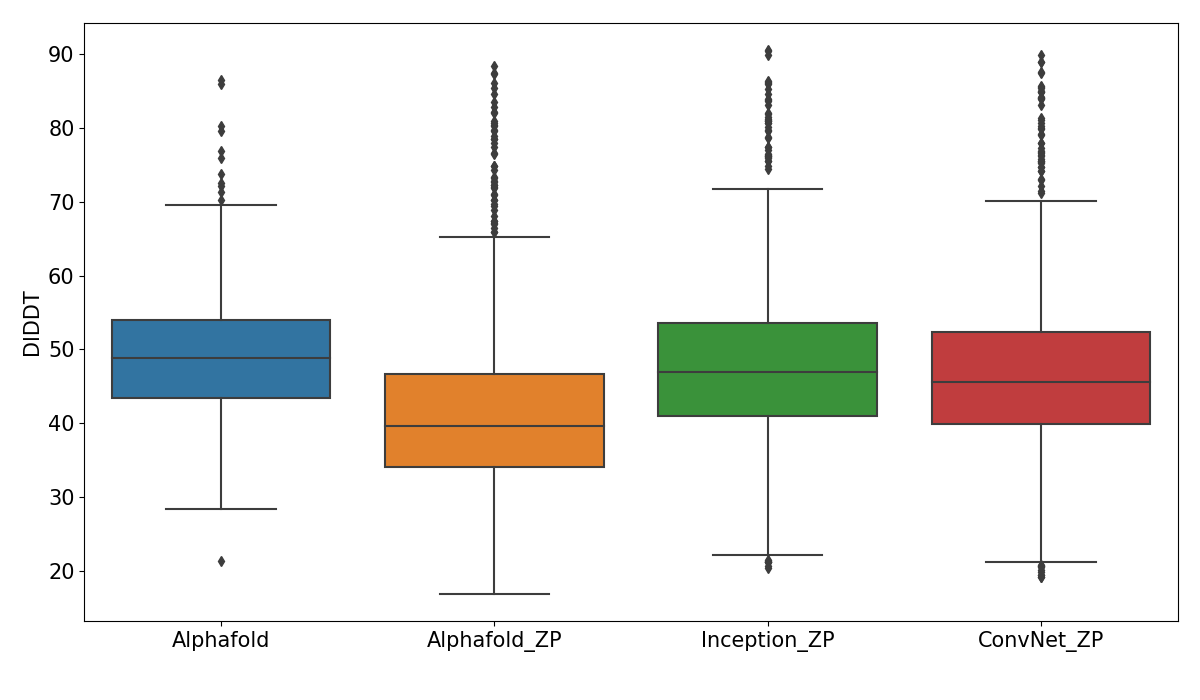
\includegraphics[width=\linewidth]{imgs_tomas/models_lddt_nice.png}
    \caption{Distogram lDDT scores calculated on the Test set for 4 different Neural Network architectures. The "ZP" abbreviation stands for Zero Padding and distinguishes the cropping schemes strategies}
    \label{fig:models_lddt}
\end{figure}

The model choice was performed on a validation set of 1000 domains, which were not used in training. Each domain was predicted by each model and its DlDDT score was calculated from the distograms (see Equation \ref{eq:dlddt}). The Figure \ref{fig:models_lddt} shows the results. 

Our initial idea was to weigh the models according to these scores. However, since they were highly correlated, we abandoned the plan and only picked the best model. The AlphaFold (with cropping scheme number 1) performed best of all models, while the Inception architecture leads the Zero-Padding group ($\Leftrightarrow$ cropping scheme number 2). Thus, the domains larger than 63 residues were predicted with AlphaFold architecture (since first cropping scheme (Figure \ref{fig:cropping}a)) does not work with domains smaller than 64 residues), and the rest with Inception\_ZP. 

\begin{figure}
    \centering
    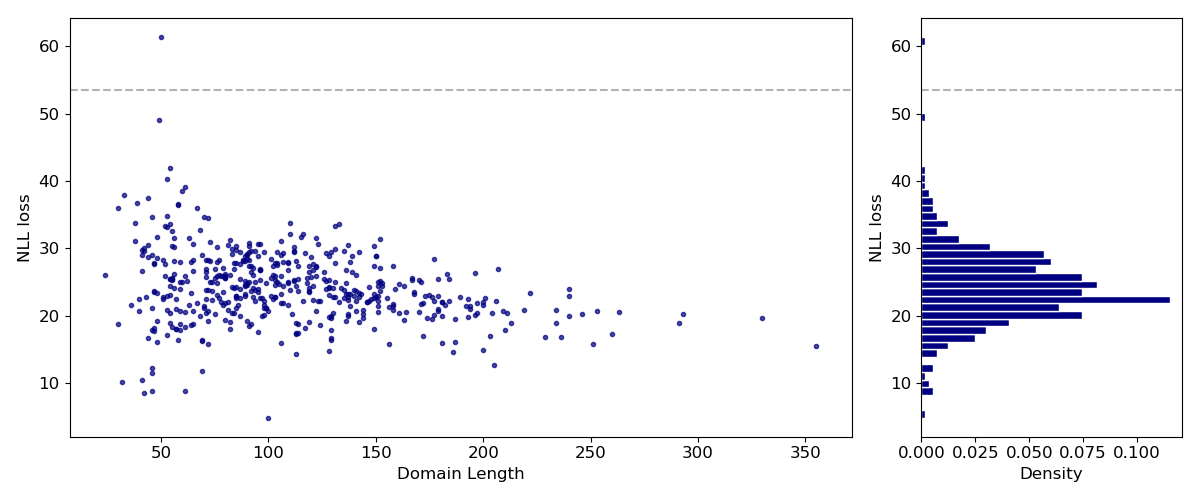
\includegraphics[width=\linewidth]{imgs_tomas/test_losses_distributions.png}
    \caption{Test loss against domain lenth together with its distributions. The NLL loss is a weighted function composed of distogram loss and auxiliary losses - see Equation \ref{eq:NLLloss}. The grey line shows the boundary between random and non-random predictions}
    \label{fig:test_losses}
\end{figure}

For a final evaluation of the model performance we used two test sets: one coming from the CATH database and then 13 domains from CASP13. Figure \ref{fig:test_losses} shows the distribution of overall losses for all CATH test domains together with domain length relationship. 

We can safely conclude that our models were able to extract important features from the input and generate non-random outputs. The boundary between the random and non-random model can be calculated from Equation \ref{eq:NLLloss}:

$$- 10~log(1/32) + 2~log(1/9) + 4~log(1 / 37) \approx 53.45$$

\begin{figure}
    \centering
    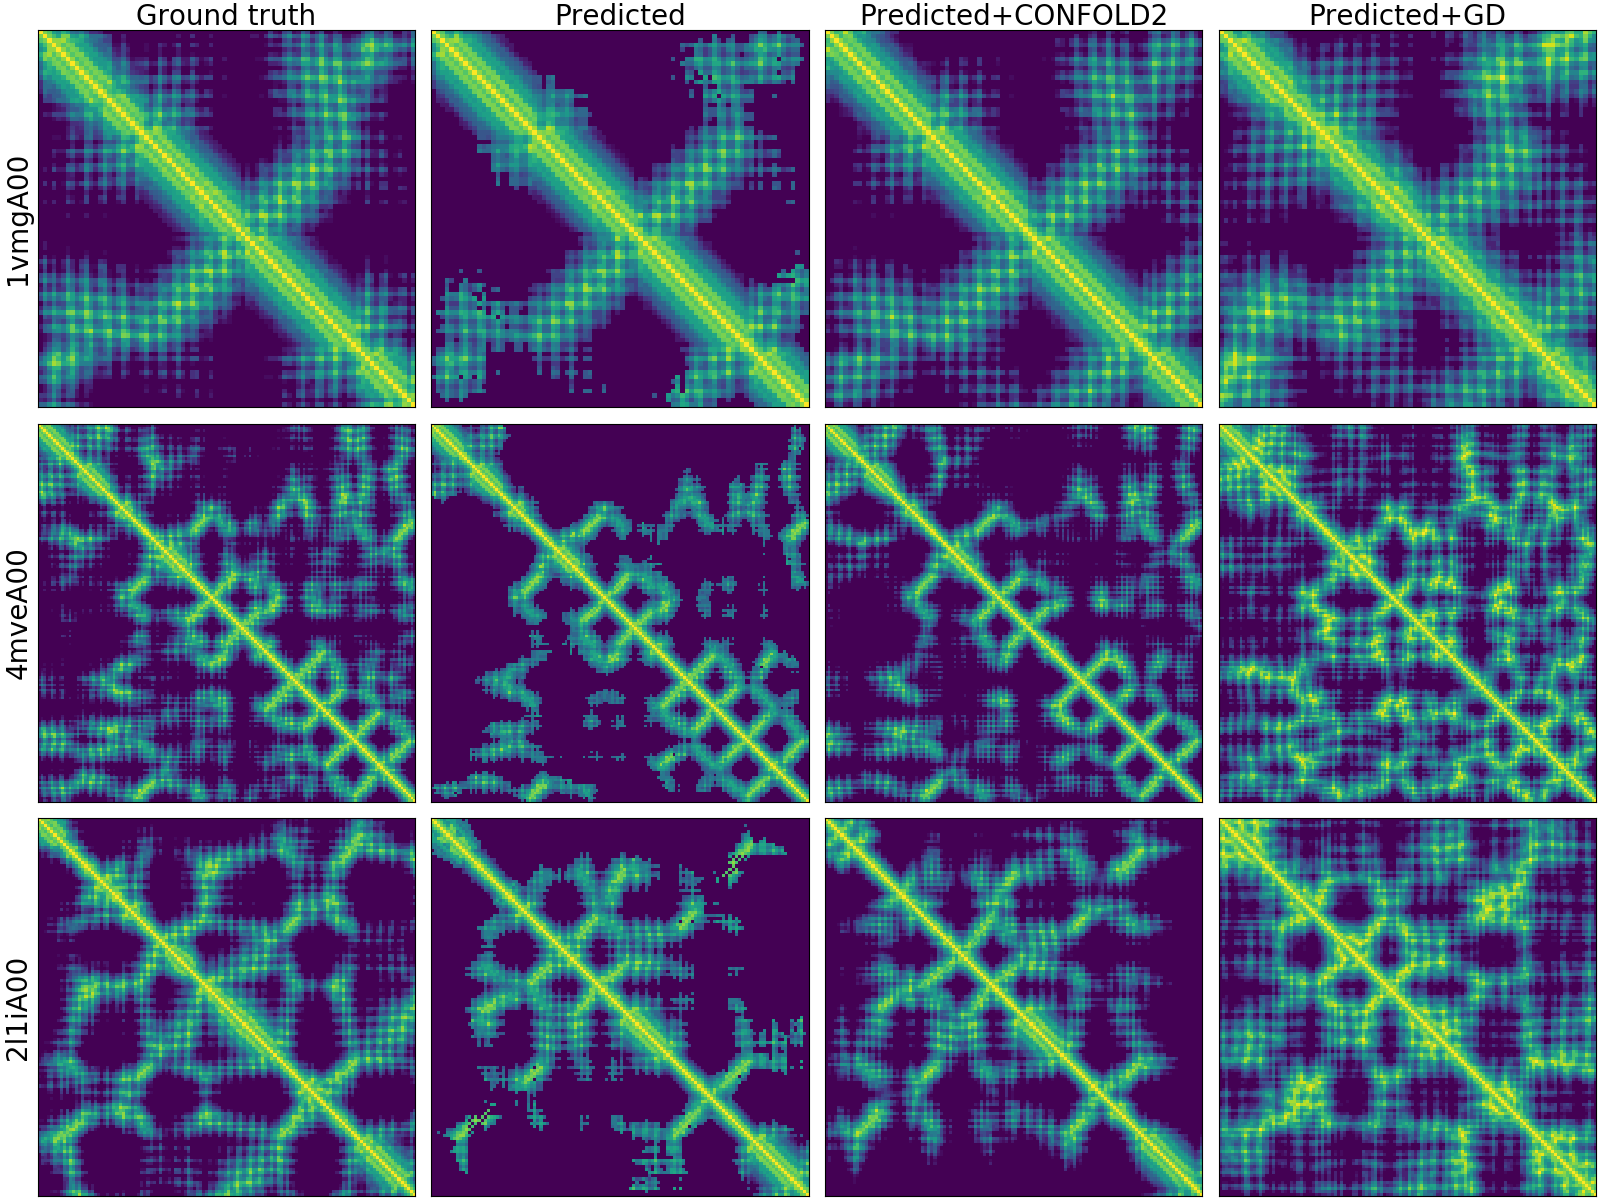
\includegraphics[width=\linewidth]{imgs_andy/distograms/distance_maps_test_structures.png}
    \caption{Comparison of ground truth and predicted distograms. We selected three proteins based on the calculated error made in their predictions. First row is a very good prediction of a protein 1vmgA00 with measured error 20.42. Only 5\% of the distograms achieved better accuracy. Second row is a prediction of protein 4mveA00 with median error amongst the test set. Third row is a prediction of protein 2l1iA00. 95\% of the errors from test set achieved better score. In all cases, the ground truth is displayed on the left and the predicted distograms on the right.}
    \label{fig:distograms}
\end{figure}

This can be also seen on the predicted distance maps shown in Figure \ref{fig:distograms} where we picked three domains based on their loss. The columns show the real distance maps, prediction derived from Neural network and induced maps from folded 3D structures using 3rd party program CONFOLD2 and our own Gradient Descent based structure optimization. The first domain respresents the fifth percentile of the loss distribution (only 5\% of domains had lower loss), middle is a median prediction and bottom represents the 95th percentile.

The first interesting point regarding the results is, that the prediction loss does not get worse for longer domains. This means, that the network was able to predict different regions of the distance maps, both on and off diagonal.

The second fact, although not so obvious as the first one, is suggested by the predicted and real distance maps in Figure \ref{fig:distograms}. Although not surprising, the network had troubles predicting finer features of the distance maps. The main patterns are almost always captured, but other than that, we observed that the network simply puts the rest of distances in the last bin (visualized as dark blue regions). One has to keep in mind, however, that input was essentialy composed of amino acid correlations in the MSA. Thus highly correlated pairs should be easily extracted and so should the uncorrelated ones. The hard task is to fill in the void between those two extreme

\begin{figure}
    \centering
    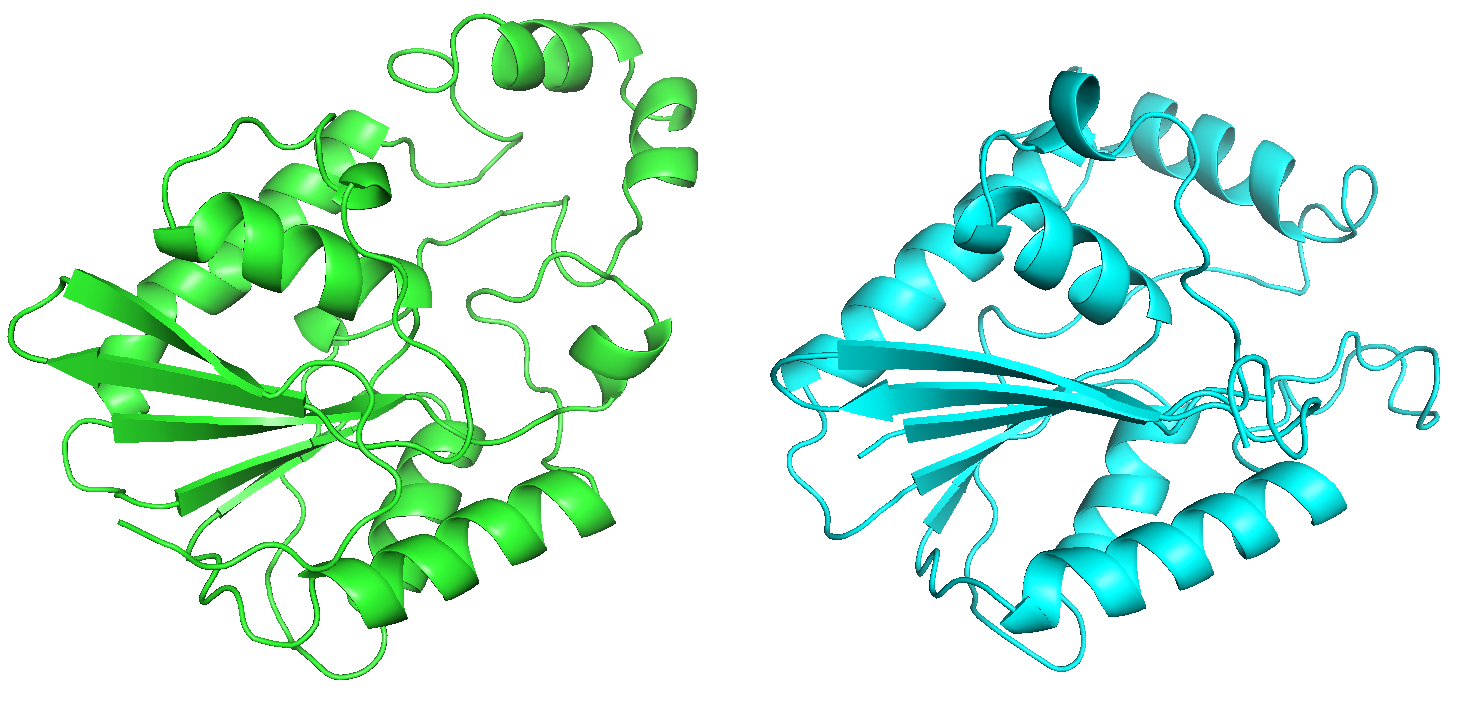
\includegraphics[width=\linewidth]{imgs_tomas/T1016_structure.png}
    \caption{Domain (T1016-D1) from CASP13 with the highest TMscore = 0.66. On the left is the real structure; on the right the one optimized by CONFOLD2}
    \label{fig:T1016}
\end{figure}

\section{Structure Realization}

\subsection{Gradient Descent Based Structure Realization}

\begin{figure}
    \centering
    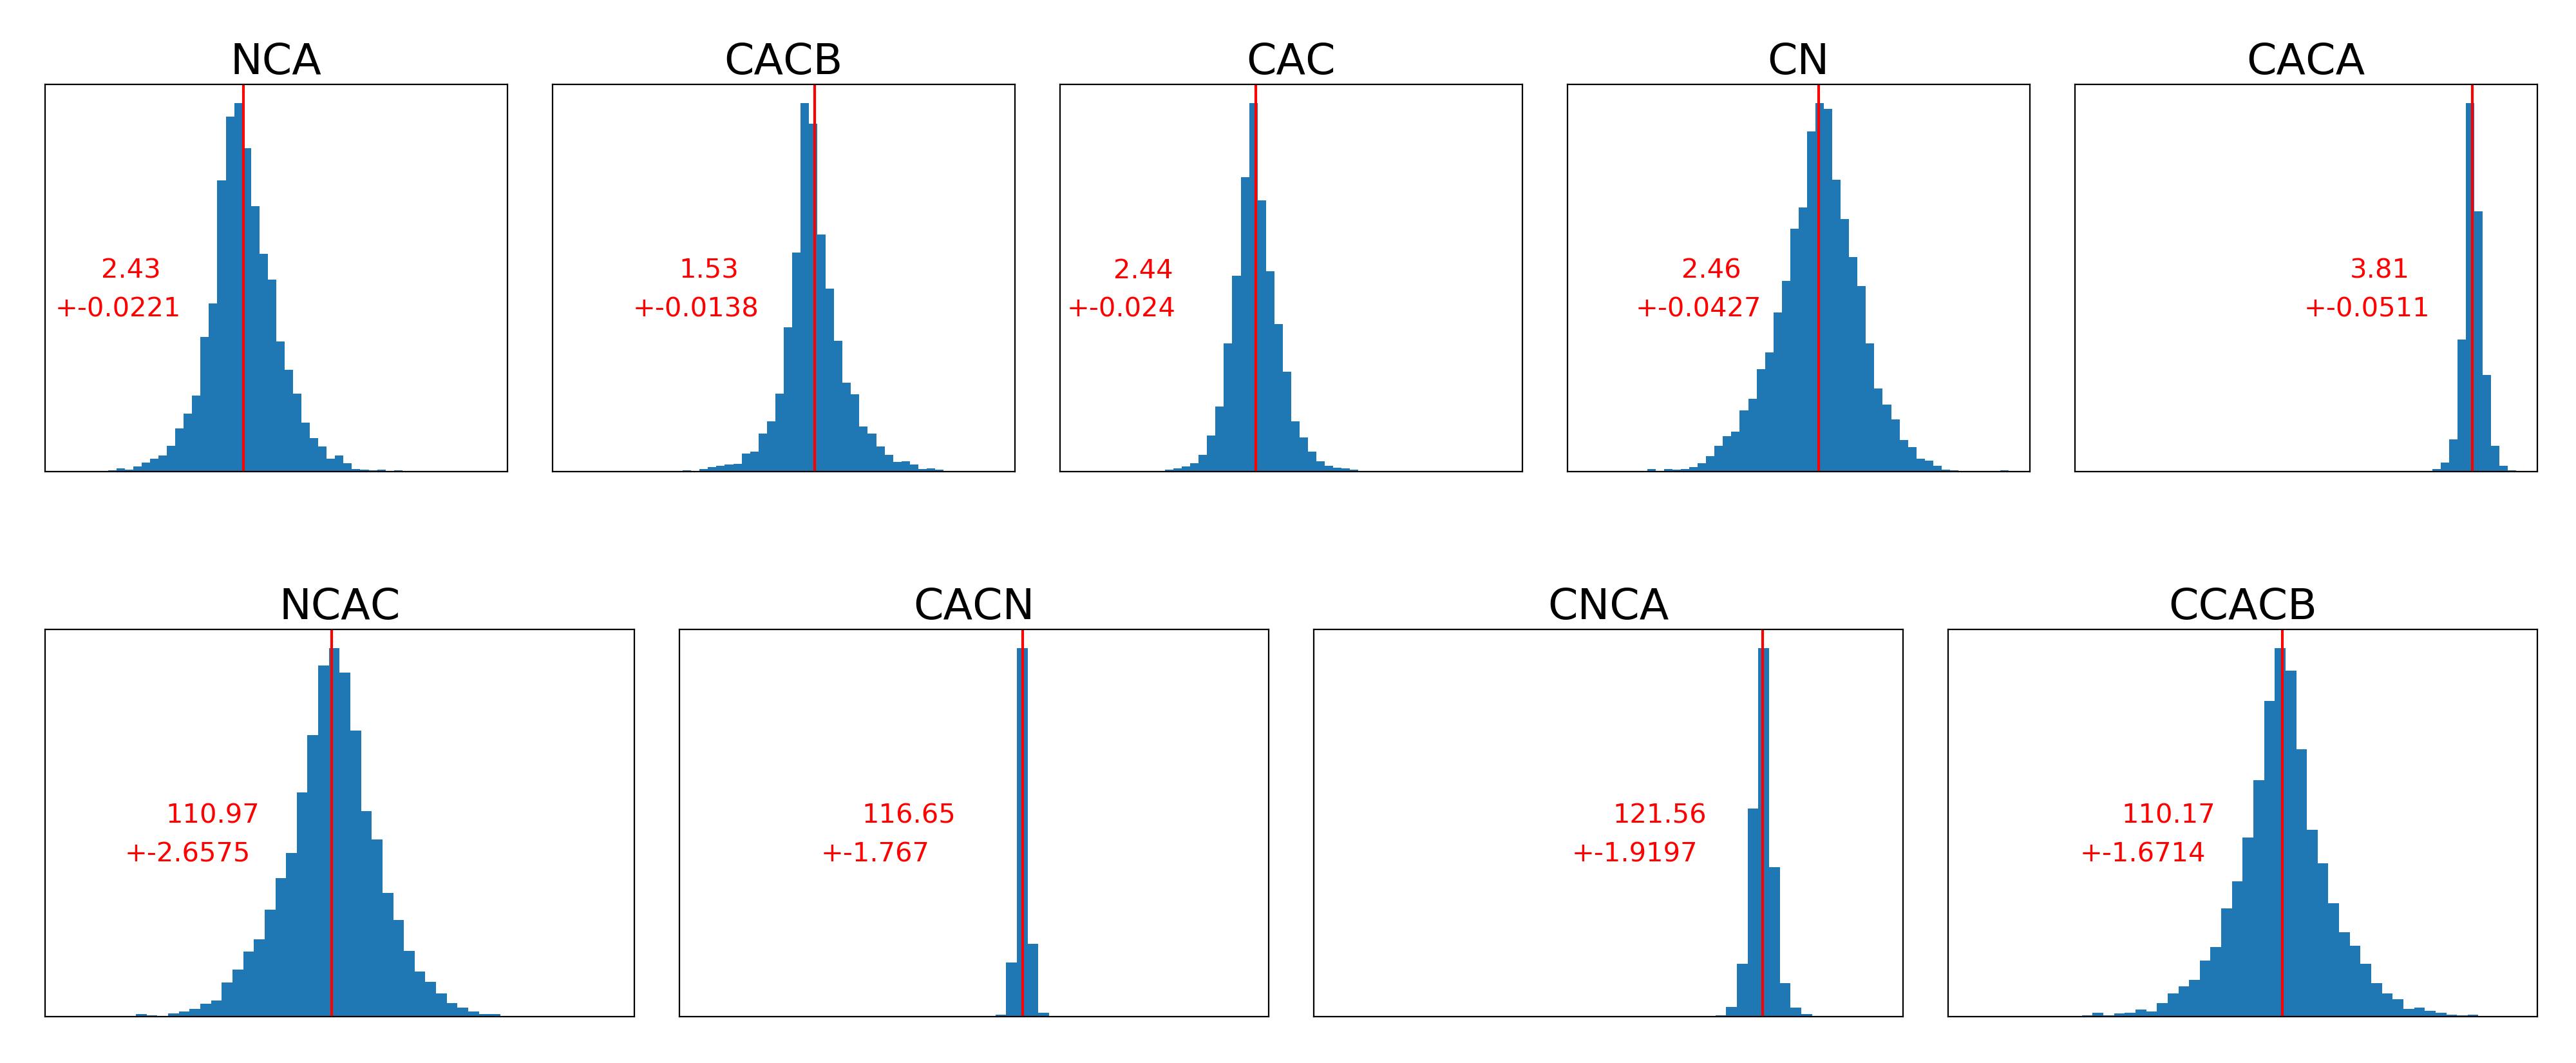
\includegraphics[width=\linewidth]{imgs_tomas/inter_data.png}
    \caption{Inter-atom distance distributions (top row) and angles defined by three consecutive atoms in a plane (bottom row) calculated from 50 protein structure downloaded from PDB. The red line represents the mean of the distribution, together with the first number in red text. The second number is the standard deviation}
    \label{fig:interresidue}
\end{figure}

\begin{figure}
    \centering
    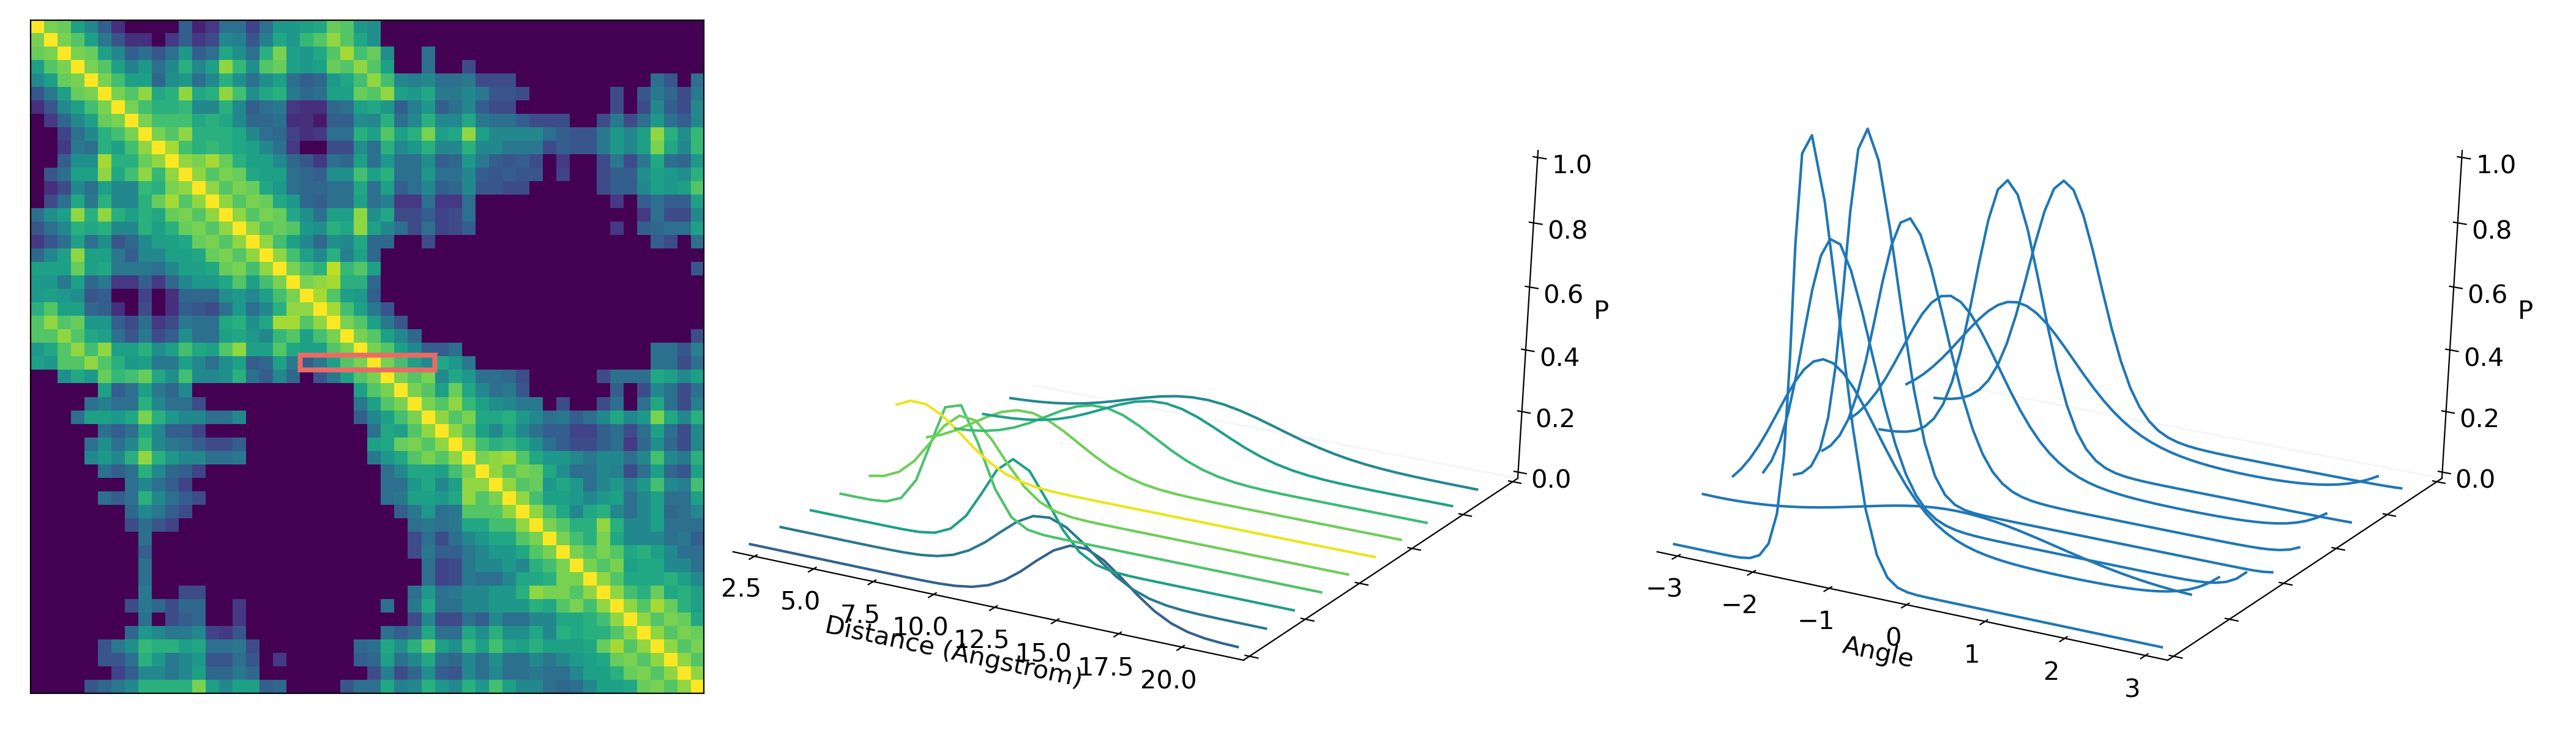
\includegraphics[width=\linewidth]{imgs_tomas/histograms2.png}
    \caption{Fitted normal distributions to the distance histograms (middle) and von Mises distributions to the angle histograms (right) to a small region of domain 16pkA01}
    \label{fig:distributions}
\end{figure}

In order to implement the model of protein geometry, one has to treat the distances between neighboring atoms in the backbone as constants, together with the angles of 3 consecutive backbone atoms. We analyzed coordinates of 50 randomly selected proteins and calculated these distances and angles; the results are shown in Figure \ref{fig:interresidue}. The means of the distributions were used in the creation of the protein geometry.

For a given structure we generated 1000 unique random initial states by sampling from the von Mises distributions fitted to the histograms. The individual distributions are depicted on Figure \ref{fig:distributions}. From each angle distribution (right of the Figure \ref{fig:distributions}) one value was picked. The normal distance distributions (Figure \ref{fig:distributions} - middle) were used for the calculation of the loss function - see Equation \ref{eq:dist_pot}.

For each torsion angle initiation we let the algorithm run for 1000 iterations. However, after every 200 iterations the algorithm picked the best structure (according to the loss) and continued the optimization with decreased learning rate (by a factor of 10).

The initial parameters were chosen by visually exploring the learning curves of 3 random states. The grid search was composed of combination of parameters:

$$learning~rate = [0.1, 0.05, 0.01. 0.005, 0.001]$$
$$momentum = [0.1, 0.3, 0.5, 0.7, 0.9]$$

In the end, we decided to use initial learning rate = 0.05 and momentum = 0.5. The idea behind these values was to let the algorithm "explore" the landscape in the first iterations, without getting stuck in some local optimum. The decreased learning rate after each iterations lets the structure optimize finer and finer elements of its geometry.

\begin{figure}
    \centering
    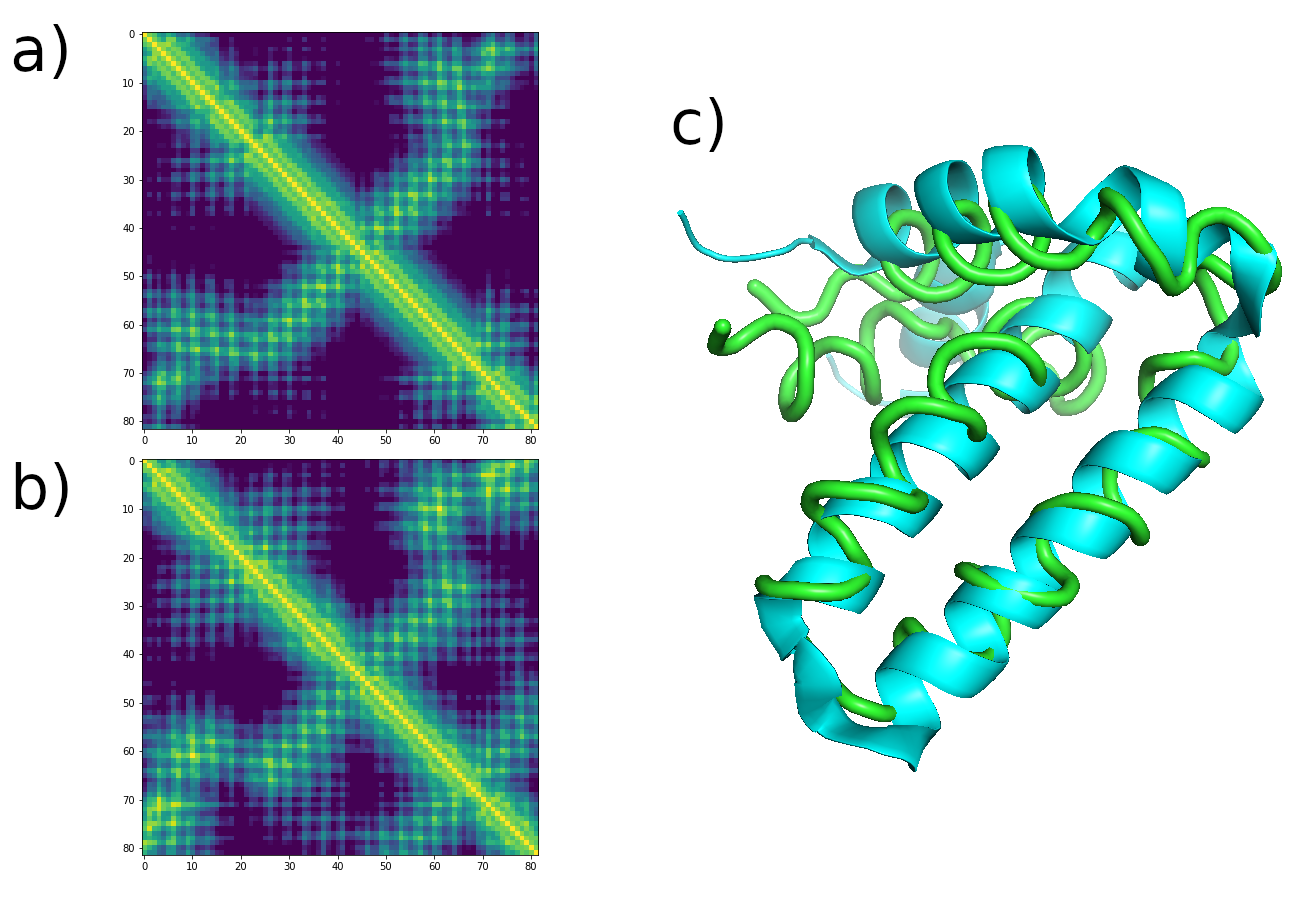
\includegraphics[width=0.8\linewidth]{imgs_tomas/1vmg_ensemble.png}
    \caption{An example of optimized structure of domain 1vmgA00 (length = 82). a) is the real (binned) distance map, b) is the distance map induced from the optimized structure and c) shows the predicted structure (green) aligned on real one (blue)}
    \label{fig:1vmg}
\end{figure}

Although the algorithm works and the distance map of the optimized structure looks similar to reality (see Figure \ref{fig:1vmg}),
its main disadvantage is that it does not punish entangled conformations, which can not occur in reality. The reason for this is that the loss function only looks at the distance map which can not hold enough information about the structure (especially if it is not a perfect prediction). The authors of the Alphafold used more complicated loss function with three terms:

\begin{equation}
    V(\phi, \psi) = V_{dist}^{ref}(\mathcal{G}(\phi, \psi)) + V_{torsion}(\phi, \psi) + V_{score2smooth}(\mathcal{G}(\phi, \psi))
    \label{eq:alphafold_potential}
\end{equation}

The first term is a distance potential similar to the one we used, but with additional step of subtracting a reference distribution in the log part of the NLL loss. The reference distribution captures the inherent noise of the network and models the relationship between the output distributions and domain length + binary feature is glycin or not.

The second term is simple NLL function where the log probability is calculated from the von Mises distributions fitted to the angle histograms.

Finally, the last term punishes the structure if steric clashes occur. This was the only function that AlphaFold team borrowed from the Rosetta commons modelling software \cite{rosettacommons}. On top of this, the authors of the AlphaFold did not use gradient descent for optimization but a more advanced method - L-BFGS (Limited memory Broyden–Fletcher–Goldfarb–Shanno) which is a method that resembles the second order optimization by estimating the Hessian matrix (matrix of second derivatives). The method does not pick directions where the loss function changes the fastest, but rather where the gradients change the fastest. This results in more reasonable steps and thus the convergence is usually reached in smaller number of steps. The biggest downside of the method is that it is slow and tends to get stuck in saddle points of the loss function \cite{nn_dl}.

Due to lack of time, we omitted the last two terms of the potential together with the reference distribution and used only the distance potential. 

One option that fixes the steric clashes is to use The Rosetta modelling software, which offers the so called FastRelax protocol. 
FastRelax takes as an input a structure in \texttt{pdb} format and performs several steps of "relaxation", where the steric clashes are fixed and the free energy of the structure is minimized. 
This is not the optimal solution, since the inter-residue distances that were optimized in the first step get slightly distorted, but the structure at least makes more sense on terms of molecular physics. 
Nevertheless, we found the program to be too strong (with its default values) because it changed the structure too much.
Therefore, until we develop a better potential function we decided to use a third party software: CONFOLD2. 
%we had to used a different software (CONFOLD2) where the optimization is based on satisfying contact map and secondary structure (Q3) constraints.

\subsection{CONFOLD2}
Another approach we used for structure realization was CONFOLD2 software.
This software takes residue contacts and secondary structure of the protein as an input and produces 5 of the best protein folds.
Therefore, we calculated the residue contacts from the distograms.
The probabilities of the first 11 bins were summed up to get a probability that the distance between residues $i$ and $j$ is less than 8 angstroms.
If the resulting probability was more than 0.5, we assumed that the residues $i$ and $j$ are in contact.
The prediction of secondary structure was acquired from the auxiliary outputs of the neural network.
Consequently, it was converted from the Q8 format to the Q3 format, because this was the format required from CONFOLD2.

The residue-residue contacts and the secondary structure information is used internally by CONFOLD2 to create constraints of the model.
Then, the 3D structure modelling is performed in two stages.
In the first stage, these constraints are used to create multiple protein models.
These protein models are then used to filter out unsatisfied constrains.
In the second stage, the remaining constraints are used to reconstruct the final models.

According to Adhikari et al. \cite{confold}, this two stage modelling significantly improves the quality of the resulting 3D structure.

\subsection{Evaluation}

\begin{figure}
    \centering
    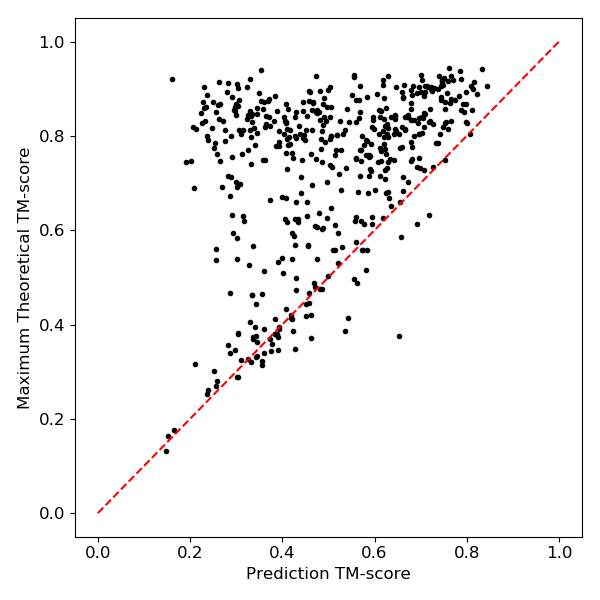
\includegraphics[width=0.6\linewidth]{imgs_tomas/test_tmscore.png}
    \caption{TM-scores of structures generated from real contact maps and secondary structures (y axis) vs TM-scores of structures optimized from predicted contact maps and secondary structures.}
    \label{fig:test_tmscore}
\end{figure}

\begin{figure}
    \centering
    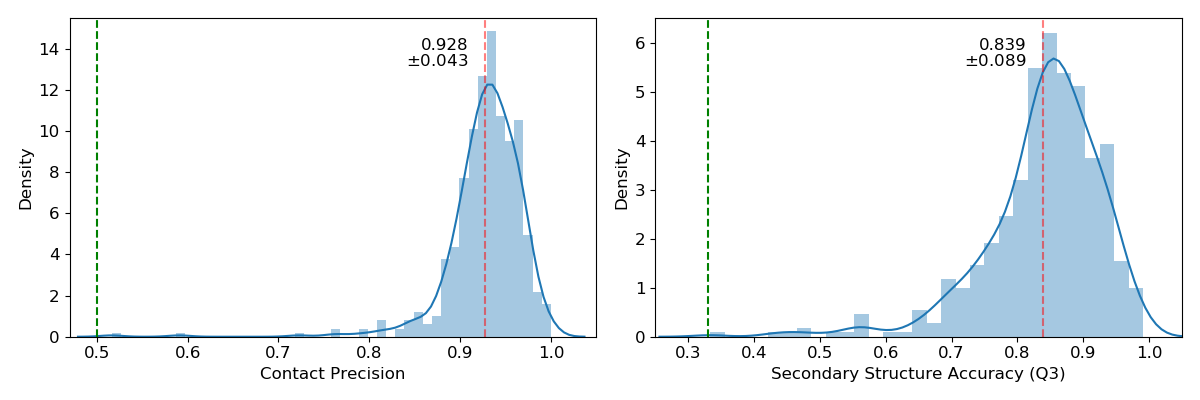
\includegraphics[width=\linewidth]{imgs_tomas/contacts_secondary_eval.png}
    \caption{Distributions of precision values for contact predictions and accuracy values for 3 state secondary structure classification, both calculated on the test set. The two values on top of the plot represent the mean (also depicted as a red dashed line) and standard deviation of the distribution. The orange line shows the performance of a random model}
    \label{fig:contacts_sec}
\end{figure}

\section{Comparison with other methods}
\subsection{Distances}
\subsection{Structures}

\begin{figure}
    \centering
    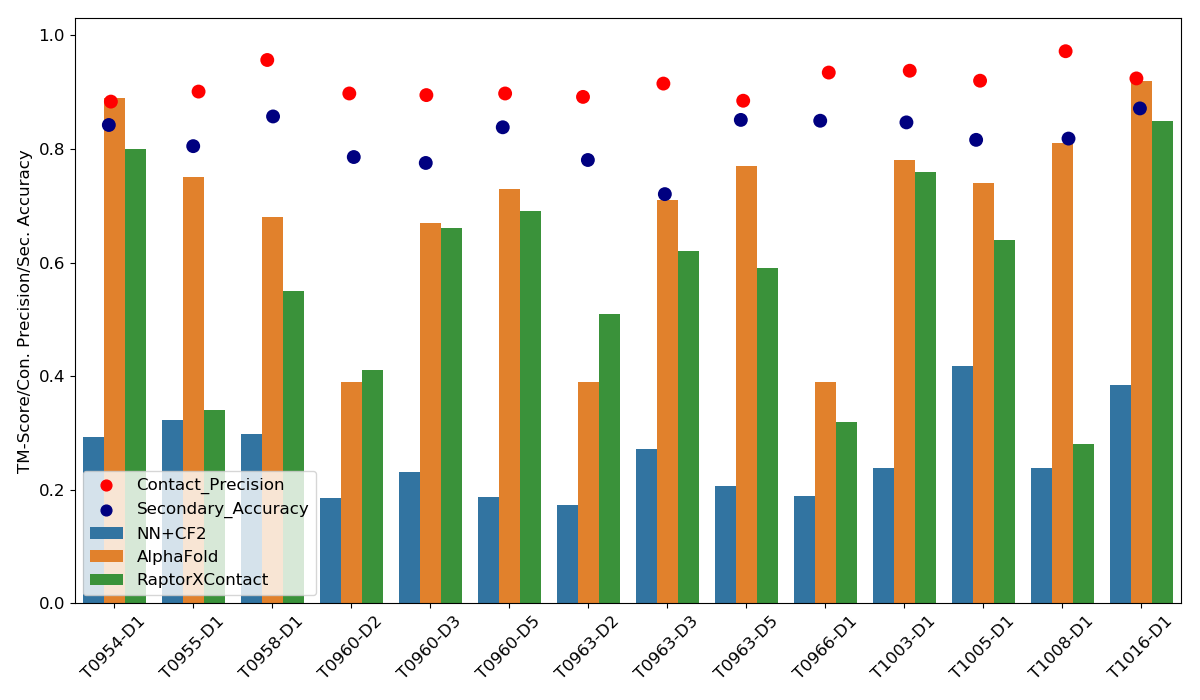
\includegraphics[width=\linewidth]{imgs_tomas/casp13_tm_contacts_sec.png}
    \caption{Performance of our Pipeline (NN + CF2) against team Alphafold and RaptorXcontact for selected targets used in CASP13. Structures with TMScores less than 0.17 (red dashed line) are not better than random folds while structures with TMscore > 0.5 (green dashed line) should have similar overall topology the real structure}
    \label{fig:casp_performance}
\end{figure}

\begin{figure}
    \centering
    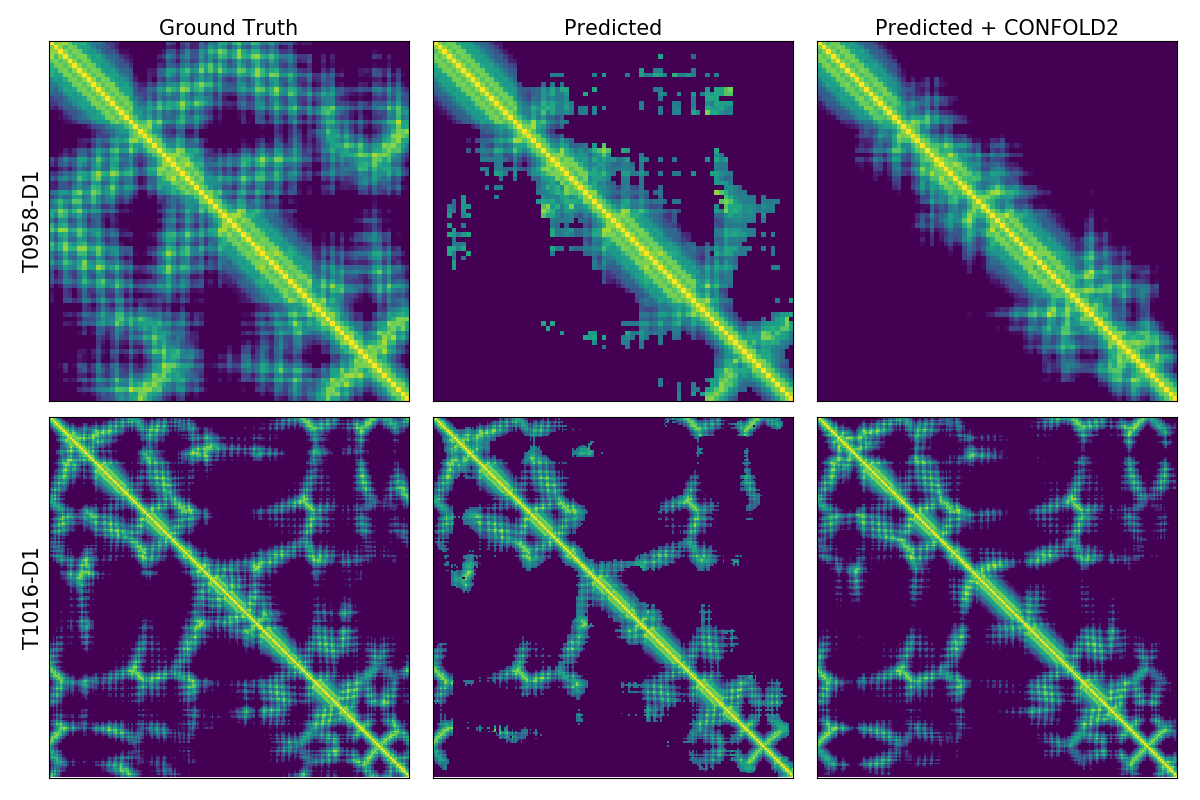
\includegraphics[width=\linewidth]{imgs_tomas/casp_distance_maps_test_structures.png}
    \caption{Distance maps of two targets from CASP13, similar to Figure \ref{fig:distograms}. For the first domain the sequence search algorithm (HHblits) only found 43 sequences from which it "constructed" the MSA (the effective number of homologs $Neff \approx 30.7$).  Unsurprisingly the neural network had a hard time and CONFOLD2 could not do much to fix this. b) shows a different scenario, when the number of sequences in MSA was adequate (1039, with $Neff \approx 1157$) and so was the neural network prediction. After CONFOLD2 folded the structure, the distance map looks even more similar to reality than predicted one}
    \label{fig:casp_distmaps}
\end{figure}

\begin{figure}
    \centering
    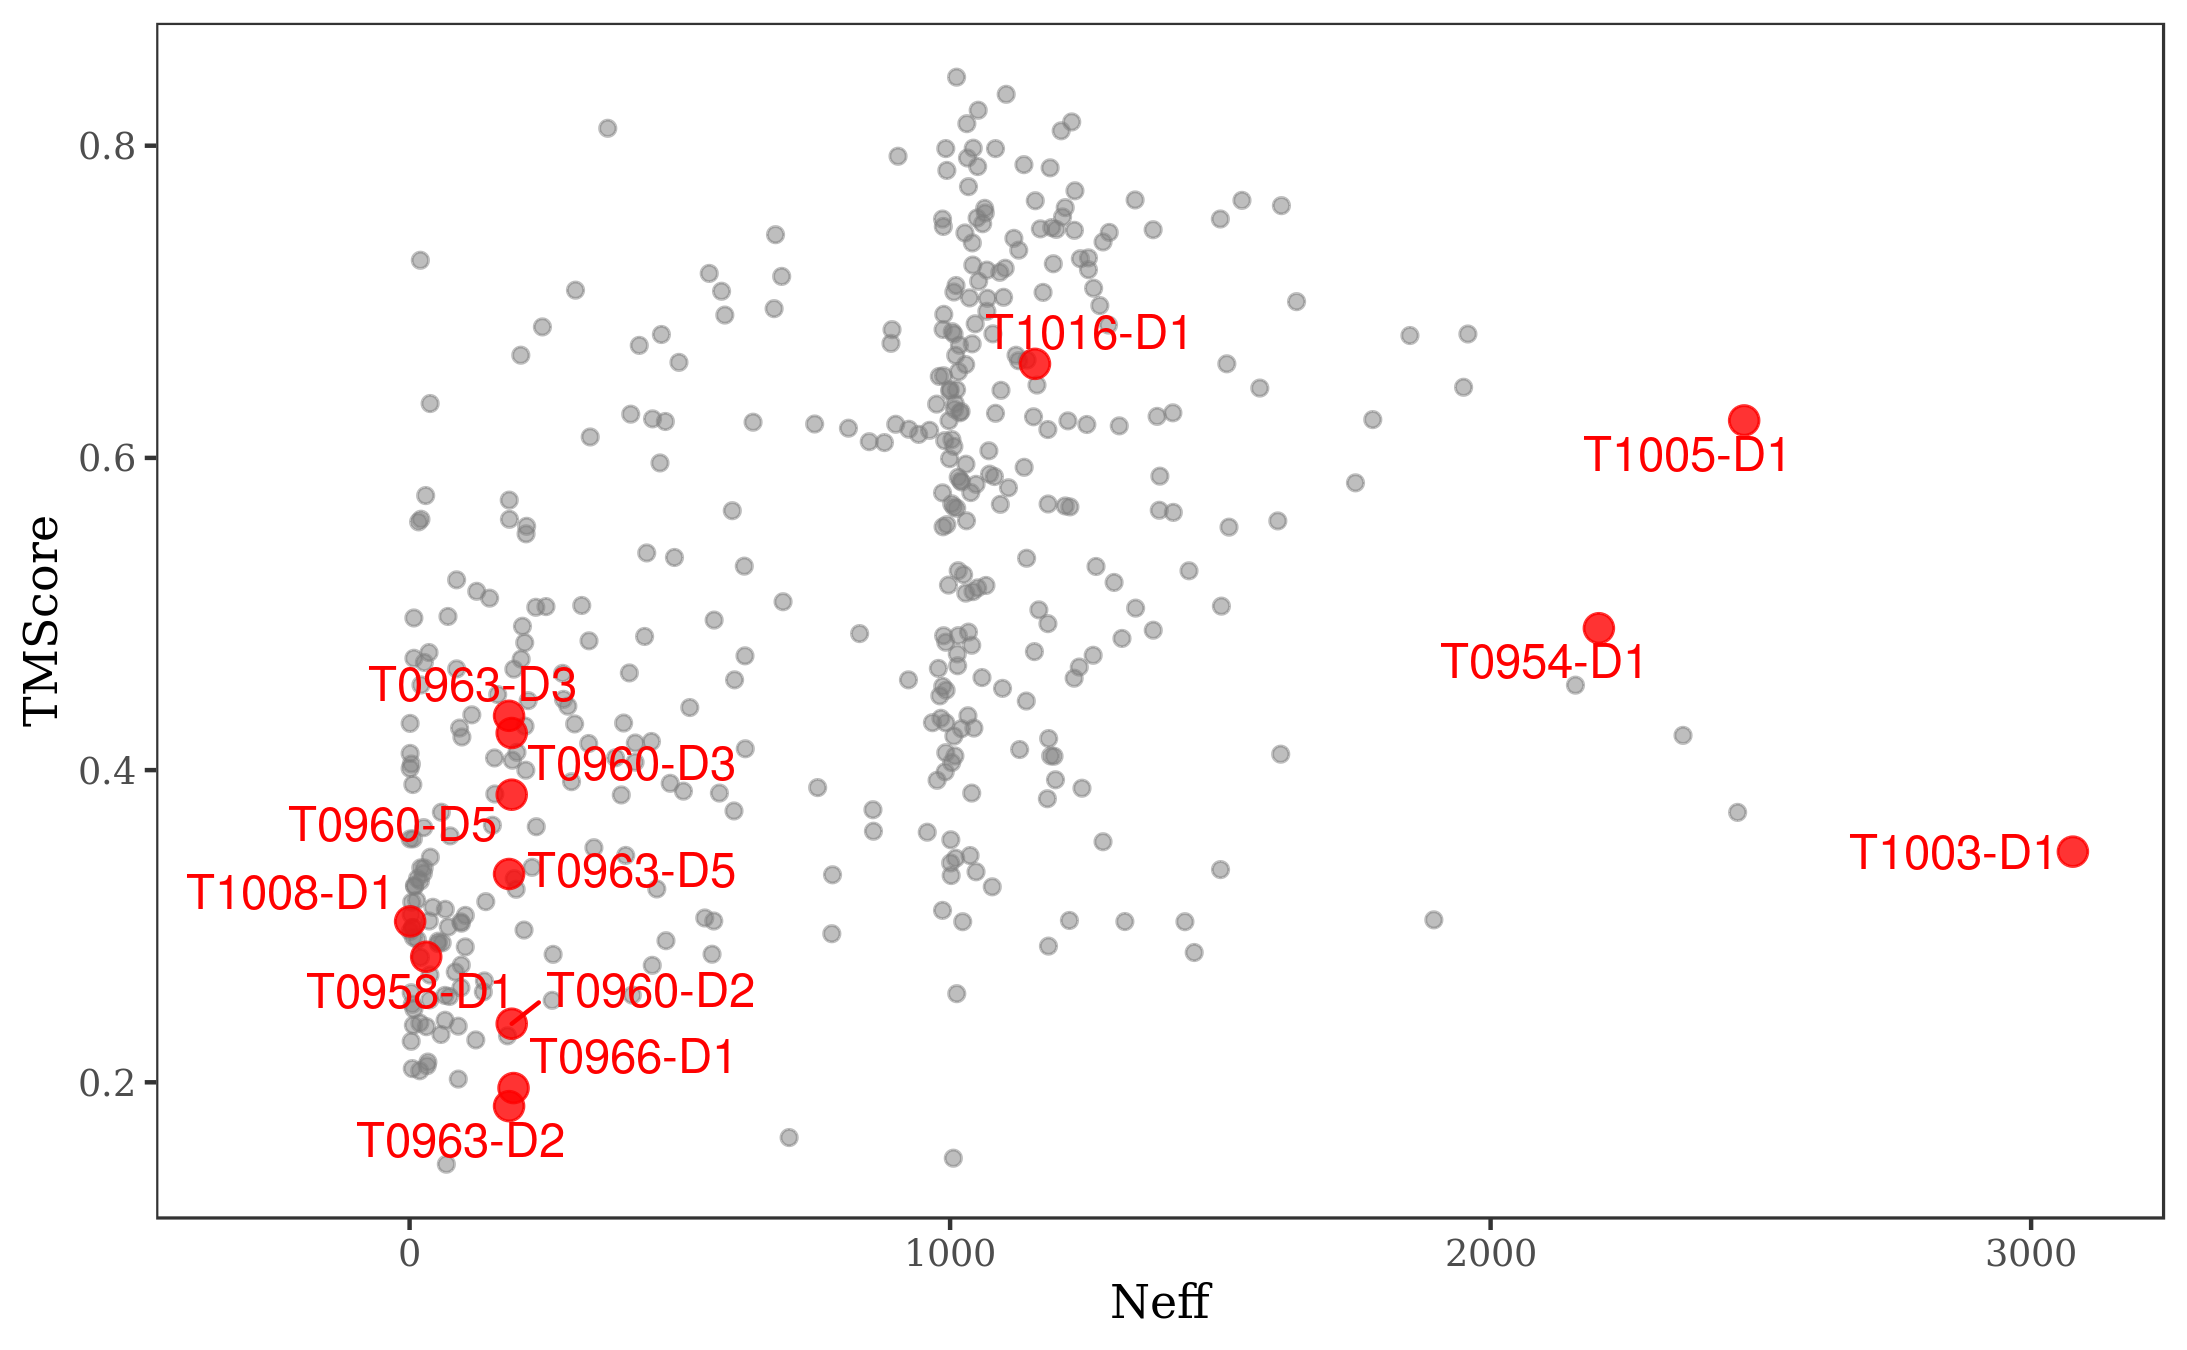
\includegraphics[width=\linewidth]{imgs_tomas/tm_vs_neff.png}
    \caption{TM score vs Number of Effective homologs (Neff) in the MSA. Grey points represent the domains from test set; red points are the CASP13 targets}
    \label{fig:tm_vs_neff}
\end{figure}

\section{Potential improvements}

\subsection{Regarding Input Data}
what to do when the protein does not have enough similar sequences in the database?
NEFF

PLMC might not converge. What are the reasons for this and how should we handle it.

Optimization of the input pipeline is needed.
HHblits and Psiblast both do a sequence search and MSA.
Ideally we would like to do this just once and then from MSA compute the PSSM and potts models.
Although it might be beneficial to do it like it is, because the input features will be less correlated to each others.

It might be beneficial to include calculated limits of the physical distance of 2 aminoacids.
For example, we know that 2 aminoacids next to each other are 3.8A away.
Similarly, 2 aminoacids at position $i$ and $i+2$ are ???5.6???A away.
For position $i$ and $i+3$ this starts t be interesting, but calculating the maximum distance and the minimum distance should be relatively easy.

Refactoring pipeline to be truly reproducible.

Using more covariance data modelling approaches, not just PSSM and potts, but also PSICOV and Bayesian networks.

\subsection{Regarding Neural Networks}
Neural networks could be modified to predict parameters of some distribution of distances.
In currect setting we are predicting distrogram characterized by 32 numbers.
If we would be able to identify some reasonable parametric distribution for distances, these could be used instead of the distrogram, reducing the number of parameters of the network and making the formulation closer to some theorethical formulation related to protein than very general.

Use accumulating gradients. This would allow to train on bigger batches than is the memory limit of the GPU and also would allow to train on multiple GPUs.
% https://medium.com/huggingface/training-larger-batches-practical-tips-on-1-gpu-multi-gpu-distributed-setups-ec88c3e51255

\subsection{Regarding Structure Realization}

Even though the algorithm for optimizing structure works, it is highly dependant on the choice of hyperparameters, which might not be ideal for every domain. 